%%%%%%%%%%%%%%%%%%%%%%%%%%%%%%%		CHAP 1		%%%%%%%%%%%%%%%%%%%%%%%%%%%%%%%

\clearpage
\chapter{Neutrinos in the Standard Model}
\label{cha:intro}

The Standard Model (SM) is a renormalisable Yang-Mills theory~\ref{} that describes the strong, electromagnetic, and weak interactions %
of elementary particles in the framework of quantum field theory.
It is based on the local gauge symmetry group 
\begin{equation}
	\label{eq:smgroup}
	\text{SU(3)}_C \otimes \text{SU(2)}_L \otimes \text{U(1)}_Y
\end{equation}
where $C$, $L$ and $Y$ denote respectively colour, left-handed chirality and weak hyper-charge.
The gauge group uniquely determines the interactions and the number of %
vector gauge bosons that correspond to the generators of the group.
%
The electroweak subgroup $\text{SU(2)}_L \otimes \text{U(1)}_Y$ undergoes a spontaneous symmetry breaking process %
out of which three of the four vector bosons acquire mass ($W^\pm$ and $Z$~bosons) and the last one, the photon, remains massless.
The colour section is unbroken and does not mix with the electroweak sector: %
the generators of the algebra of $\text{SU(3)}_C$ corresponds to eight massless gluons.
%
%%In the SM, electroweak interactions can be studied separately from strong interactions, %
%%because the symmetry under the color group is unbroken and there is no mixing %
%%between the SU(3)$_C$ and the $\mathrm{SU(2)}_L \otimes \mathrm{U(1)}_Y$ sectors.
%%On the other hand, the Glashow, Salam, and Weinberg theory well explains the group mixing between %
%%electromagnetic and weak interactions caused by a symmetry breaking process.
%%They are eight massless gluons that mediate strong interactions, %
%%corresponding to the eight generators of SU(3)$_C$, and four gauge bosons, %
%%of which three are massive ($W^\pm$ and $Z$) and one is massless, corresponding %
%%to the three generators of SU(2)$_L$ and one generator of U(1)$_Y$, responsible for %
%%electroweak interactions.
Since the number and properties of the gauge bosons is determined by the SM group, %
the only independent parameters left are the coupling constants of the interactions, which can be determined by the experiments.
The spontaneous breaking symmetry requires at least one scalar boson thanks to the Higgs mechanism.
The recent discovery of the Higgs boson is the crowning achievement of the SM~\ref{}.
%The symmetry group of the SM fixes the interactions, i.e. the number and properties of the %
%vector gauge bosons, with only three independent unknown parameters: the three coupling constants of %
%the SU(3)$_C$, SU(2)$_L$, and U(1)$_Y$ groups, all of which must be determined from experiments.
On the contrary, the number and properties of scalar bosons and fermions are left unconstrained, %
except for the fact that they must transform according to the representations of the symmetry group, %
while the fermion representations must lead to the cancellation of quantum anomalies.

The known elementary fermions are divided in two categories, quarks and
leptons.
They are distinguished by the fact that quarks participate in all the interactions % 
whereas leptons participate only in the electroweak interactions.
\begin{center}
	\small
	\begin{tabular}{lccc}
		\toprule
		\textbf{Generation}	&\textbf{1st}	& \textbf{2nd}	& \textbf{3rd}	\\
		\midrule
		\multirow{2}*{Quark} & $u$ 		& $c$		& $t$		\\
		& $d$		& $s$		& $b$		\\
		\midrule
		\multirow{2}*{Leptons}	& $e$ 		& $\mu$		& $\tau$	\\
		& $\nu_e$	& $\nu_\mu$	& $\nu_\tau$	\\
		\bottomrule
	\end{tabular}
\end{center}

%In the SM, electroweak interactions can be studied separately from strong interactions, %
%because the symmetry under the color group is unbroken and there is no mixing %
%between the SU(3)$_C$ and the $\mathrm{SU(2)}_L \otimes \mathrm{U(1)}_Y$ sectors.
%On the other hand, the Glashow, Salam, and Weinberg theory well explains the group mixing between %
%electromagnetic and weak interactions caused by a symmetry breaking process.
%This model and the discovery of the predicted $W$ and $Z$ bosons, in addition to the gluon, %
%the top, and charm quarks, made the fortune of the Standard Model.
%Their redicted properties were experimentally confirmed with good precision and %
%the recent discovery of the Higgs Boson is the last crowning achievement of SM.

Despite being the most successful theory of particle physics to date, the SM is actually limited %
in its approximation to reality, in that some clear evidences cannot be explained.
The most outstanding breakthrough is the neutrino oscillations, which was awarded the Nobel Prize in Physics in 2015 %
and has proved that the neutrinos are not all massless, as it is assumed by theory.
Mass terms for the neutrinos can be included in the SM, with the implications of theoretical problems.
Likewise, the SM is unable to provide an explanation of the observed asymmetry between matter and anti-matter.
It was noted by Sakharov that a solution to this puzzle would require some form of C and CP violation %
in the early Universe, along with Baryon number violation and out-of-equilibrium interactions.
These facts suggest that the Standard Model is not a complete theory and additional physics %
Beyond the Standard Model (BSM) is required.

The study of neutrinos is for sure one of the most promising probe to BSM physics and %
is of vital importance to the future development of particle physics, %
in particular through precision measurement of their interactions.
A deep understanding of neutrino interactions, and neutrino-nucleon interactions in particular, %
could lead to a great impact on long-baseline experiments, proton decay search, and supernova detection.
Since the SM is a renormalisable theory, even its quantum corrections are insensitive to the physics beyond the SM.
Because of this reason, the SM is phenomenologically very successful and so far has been able to describe all the known
phenomena, except for the indications in favour of neutrino oscillations that we will discuss in the following chapters.

\section{Electroweak sector}
\label{sec:ew_sector}

The electroweak (EW) sector of the SM is formed by the direct product of the weak isospin group $\text{SU(2)}_L$ and %
the hyper-charge group $\text{U(1)}_Y$.
The two groups are connected by the Gell-Mann--Nishijima relation which connects the $I_3$ component of the %
weak isospin operator and the hyper-charge operator $Y$  with the charge operator $Q$ as
\begin{equation}
	\label{eq:gellmann}
	Q = I_3 + \frac{Y}{2}\ .
\end{equation}
Left-handed chiral components of the fermion fields form doublets under $\text{SU(2)}_L$
\begin{equation}
	\label{eq:doublets}
	\bs{L}_L = \mqty(\bs{\nu}_L \\ \bs{\ell}_L) \quad, \quad
	\bs{Q}_L = \mqty(\bs{q}_L^U \\ \bs{q}_L^D) \ ,
\end{equation}
where the left-handed fields in bold-face represent the fermion families
\begin{equation}
	\bs{\nu}_L  = \mqty(\nu_{eL} \\ \nu_{\mu L} \\ \nu_{\tau L}) \quad , \quad
	\bs{\ell}_L = \mqty(e_L \\ \mu_L \\ \tau_L) \quad , \quad
	\bs{q}^D_L  = \mqty(d_L \\ s_L \\ b_L) \quad \text{, and} \quad
	\bs{q}^U_L  = \mqty(u_L \\ c_L \\ t_L)\ .
\end{equation}
%$\bs{q}^U$ and $\bs{q}^D$ represent respectively the up quark and down quark families.
The right-handed fields, instead, transform simply as singlets and they are
\begin{equation}
	\bs{\ell}_R = \mqty(e_R \\ \mu_R \\ \tau_R) \quad , \quad
	\bs{q}^D_R  = \mqty(d_R \\ s_R \\ b_R) \quad \text{, and} \quad
	\bs{q}^U_R  = \mqty(u_R \\ c_R \\ t_R)\ .
\end{equation}
Note that the right-handed components of the neutrino fields, $\nu_{\alpha R}$, are not historically considered in the SM %
because the neutrinos were believed massless until recent times~\ref{}.
As such, neutrinos are assumed to be massless in the SM.
The EW Lagrangian is therefore the most general renormalisable Lagrangian invariant %
under the local symmetry $\text{SU(2)}_L \otimes \text{U(1)}_Y$:
\begin{align}
	\label{eq:ew_lagrangian}
	\mathcal{L}_\text{EW} =\  &i\, \cj{\bs{L}}_L\, \sh{D}\, \bs{L}_L + i\, \cj{\bs{Q}}_L\, \sh{D}\, \bs{Q}_L + %
			 i\, \cj{\bs{\ell}}_R\, \sh{D}\, \bs{\ell}_R + i\, \cj{\bs{q}}^D_R\, \sh{D}\, \bs{q}^D_R + %
			 i\, \cj{\bs{q}}^U_R\, \sh{D}\, \bs{q}^U_R \notag \\ 
			&-\frac{1}{4} B_{\mu\nu} B^{\mu\nu} - \frac{1}{4} \vb{A}_{\mu\nu} \vb{A}^{\mu\nu} 
		      + (D_\mu H)^\dagger (D^\mu H) - \mu^2 H^\dagger H - \lambda (H^\dagger H)^2  \notag \\
		      &- \qty( \cj{\bs{L}}_L\, Y^\ell H \,\bs{\ell}_R 
		      	     + \cj{\bs{Q}}_L\, Y^D    H \,\bs{q}^D_R 
		      	     + \cj{\bs{Q}}_L\, Y^U    \widetilde{H}\, \bs{q}^U_R \ +\ \text{h.c.})\ ,
\end{align}
where the covariant derivative is defined as 
\begin{equation}
	\label{eq:covariant}
	D_\mu = \pd_\mu + i g\, \vb{A}_\mu \cdot \vb{I} + i g'\, B_\mu \frac{Y}{2}\ ,
\end{equation}
and satisfies gauge invariance, %
and $\widetilde{H} = i \sigma_2 H^*$ is the conjugate Higgs field. % thanks to the transformations
It is important to note that Dirac mass terms for fermion fields other than neutrinos %
are anyway forbidden by the gauge symmetry.
These terms will become manifest once the symmetry is broken through the Higgs mechanism (see \refsec{sec:ew_higgs}).
%\begin{align}
%	\label{eq:gauge}
%	\vb{A}_\mu \cdot \vb{I} \longmapsto 
%\end{align}
The vector boson fields $\vb{A}^\mu = (A_1^\mu, A_2^\mu, A_3^\mu)$ and $B^\mu$ corresponds respectively %
to the three generators $\vb{I} = (I_1, I_2, I_3)$ of the $\text{SU(2)}_L$ group %
and the generator $Y$ of the $\text{U(1)}_Y$ group.
The $\text{SU(2)}_L$ generators are $I_a = \sigma_a / 2$, where $\sigma_a$ are the Pauli matrices, %
and thus satisfy the commutation relation
\begin{equation}
	\label{eq:generators}
	[I_a, I_b] = i \varepsilon_{a b c} I_c\ ,
\end{equation}
with $\varepsilon_{a b c}$ the Levi-Civita tensor.

\subsection{Electroweak interactions}
\label{sec:ew_interactions}

Expanding the covariant derivative and ignoring the kinetic terms, we can retrieve the interaction term %
for the leptonic sector
\begin{equation}
	\label{eq:interaction}
	\mathcal{L}_\text{int} = -\frac{1}{2} \sum_\alpha %
		\mqty(\cj{\nu}_{\alpha L} & \cj{\ell}_{\alpha L}) %
		\mqty( g \sh{A}_3 - g' \sh{B} & g(\sh{A}_1 - i \sh{A}_2) \\
		       g(\sh{A}_1 + i \sh{A}_2) & - g \sh{A}_3 - g' \sh{B}  ) %
		\mqty(\nu_{\alpha L} \\ \ell_{\alpha L} ) + g'\, \cj{\ell}_{\alpha R}\, \sh{B} \, \ell_{\alpha R}\ ,
\end{equation}
where $\alpha$ is a family generation index.
Defining the combinations
\begin{align}
	\label{eq:fields}
	W^\mu &= \flatfrac{\qty(A_1^\mu - i A_2^\mu)}{\sqrt{2}} \\
	Z^\mu &= \cos \vartheta_\text{W} A_3^\mu - \cos \vartheta_\text{W} B^\mu \\
	A^\mu &= \sin \vartheta_\text{W} A_3^\mu + \cos \vartheta_\text{W} B^\mu \ ,
\end{align}
the electromagnetic field $A^\mu$ is expressed as a rotation of $A_e^\mu$ and $B^\mu$, thus recovering QED; %
the new field $Z^\mu$ also describes a neutral current process.
The Lagrangian in \refeq{eq:interaction} can therefore be divided into two parts, %
$\mathcal{L}_\text{int} = \mathcal{L}^{(CC)} + \mathcal{L}^{(NC)}$, %
describing charged-current (CC) and neutral-current (NC) interactions.
These are
\begin{equation}
	\label{eq:currents_ccnc}
	\mathcal{L}_\text{CC,L} = -\frac{g}{2\sqrt{2}}\ j^\mu_\text{CC,L} W_\mu + \text{h.c.} 
	\quad \text{and} \quad
	\mathcal{L}_\text{NC,L} = -\frac{g}{2\cos\vartheta_\text{W}}\ j^\mu_\text{NC,L} Z_\mu
		     + g\sin\vartheta_\text{W}\  \cj{\bs{\ell}}\, \sh{A}\, \bs{\ell} \ ,
\end{equation}
where the $W$ and $Z$ vector bosons have been factorised out, leaving the fermionic currents
\begin{align}
	\label{eq:lepton_cc}
	j^\mu_\text{CC,L} &= \cj{\bs{\nu}}\, \gamma^\mu(1-\gamma^5)\, \bs{\ell} \\
	\label{eq:lepton_nc}
	j^\mu_\text{NC,L} &= \cj{\bs{\nu}}\, \gamma^\mu\, (g^\nu_V - g^\nu_A \gamma^5)\, \bs{\nu} + %
		      \cj{\bs{\ell}}\, \gamma^\mu\, (g^\ell_V-g^\ell_A\gamma^5)\, \bs{\ell}\ .
\end{align}
The constant $g'$ has been re-written in terms of $g$ and $\vartheta_\text{W}$ by setting to zero the coupling of neutrinos %
to the electromagnetic field for neutrinos, which gives
\begin{equation}
	g \sin \vartheta_\text{W} = g' \cos \vartheta_\text{W}\ .
\end{equation}
Another important relation comes from the charged lepton couplings with the electromagnetic field which must coincide %
the QED Lagrangian: we have that $g \sin\vartheta_\text{W} = q_e$ and so $g^2 + g'^2 = q_e^2$.
The~constants $g_V$ and $g_A$, introduced in \refeq{eq:lepton_nc}, can be defined for any fermion $f$ as
\begin{equation}
	\label{eq:gv_ga}
	g_V^f = I_3^f - 2 q^f \sin^2 \vartheta_\text{W} \quad \text{and} \quad
	g_A^f = I_3^f\ .
\end{equation}
Thanks to this notation, the interaction Lagrangian for the quark sector can be written in the same form of %
\refeq{eq:currents_ccnc}, where the fermionic currents of \refeqs{eq:lepton_cc}{eq:lepton_nc} now become
\begin{align}
	\label{eq:quark_cc}
	j^\mu_\text{CC,Q} &= \cj{\bs{q}}^U\, \gamma^\mu(1-\gamma^5)\, \bs{q}^D \\
	\label{eq:quark_nc}
	j^\mu_\text{NC,Q} &= \cj{\bs{q}}^U\, \gamma^\mu\, (g^U_V - g^U_A \gamma^5)\, \bs{q}^U + %
		      \cj{\bs{q}}^D\, \gamma^\mu\, (g^D_V-g^D_A\gamma^5)\, \bs{q}^D\ .
\end{align}

\subsection{Higgs mechanism}
\label{sec:ew_higgs}

In the EW Lagrangian in \refeq{eq:ew_lagrangian}, the Higgs $H$ is a complex scalar field and an $SU(2)_L$ doublet %
\begin{equation}
	\label{eq:higgs}
	H(x) = \mqty( H^+(x) \\ H^0(x) ) \ ,
\end{equation}
the potential of which can spontaneously break if $\lambda > 0$ and $\mu^2 < 0$, in
\begin{equation}
	\label{eq:higgs_potential}
	V(H) = \mu^2 H^\dagger H + \lambda (H^\dagger H)^2 \ .
\end{equation}
Defining
\begin{equation}
	\label{eq:vev}
	v \equiv \sqrt{- \frac{\mu^2}{\lambda}}\ ,
\end{equation}
the potential $V(H)$ shows a minimum for $H^\dagger H = v^2 / 2$, which %
corresponds to the lowest energy state, or vacuum.
In general, fermion and non-zero spin boson fields must have a vanishing vacuum expectation value (vev), %
so as to to preserve the Lorentz symmetries of space and time.
The same applies to charged scalar fields, as the vacuum is electrically chargeless.
On the other hand, neutral scalar fields can have a nonzero value in vacuum, and so the vev %
of the Higgs field could be given by
\begin{equation}
	\expval{H} = \frac{1}{\sqrt{2}} \mqty( 0 \\ v )\ .
\end{equation}
This value spontaneously breaks the EW group $\text{SU(2)}_L \times \text{U(1)}_Y$, %
but it remains invariant under the gauge transformations from the $\text{U(1)}_Q$ group, %
with $Q$ from \refeq{eq:gellmann}, which guarantees the existence of a massless gauge boson %
associated with the photon.
We can expand the scalar field around its vev and by choosing the unitary gauge three of the four real scalar fields %
can be rotated away being unphysical, simplifying to
\begin{equation}
	\label{eq:vev_higgs}
	\expval{H} = \frac{1}{\sqrt{2}} \mqty( 0 \\ v + h(x) )\ .
\end{equation}
Using the definition of the EW fields in \refeq{eq:fields}, %
the covariant derivative of \refeq{eq:covariant} applied to the Higgs is 
\begin{equation}
	\label{eq:d_higgs}
	D_\mu H(x) = \frac{1}{\sqrt{2}} %
		\mqty ( i \frac{g}{\sqrt{2}} W_\mu (x) \qty[v + h(x)] \\ %
			\pd_\mu h(x) - i \frac{g}{2\cos \vartheta_\text{W}} Z_\mu(x) [v+h(x)] )\ .
\end{equation}
The Lagrangian terms with the Higgs field therefore becomes 
\begin{align}
	\label{eq:all_higgs}
	\mathcal{L}_\text{Higgs} =&\ \frac{1}{2} (\pd h)^2 - v^2 \lambda h^2 - \lambda h^3 - \frac{\lambda}{4} h^4 + %
			\frac{g^2 v^2}{4} W^\dagger_\mu W^\mu + \frac{g^2 v^2}{8\cos^2\vartheta_\text{W}} Z_\mu Z^\mu \notag \\
			& +\frac{g^2 v}{2} W^\dagger_\mu W^\mu h +\frac{g^2 v}{4\cos^2\vartheta_\text{W}} Z_\mu Z^\mu h 
			 +\frac{g^2}{4} W^\dagger_\mu W^\mu h^2 +  \frac{g^2}{8\cos^2\vartheta_\text{W}} Z_\mu Z^\mu h^2\ .
\end{align}
The second term of the first line is a mass term for the scalar fields, %
from which the mass of the Higgs boson is determined to be $m_H = v \sqrt(2\lambda) = \sqrt{-2 \mu^2}$. %,
%a value recently measured~\ref{}.
The fifth and sixth terms represent the mass terms for the $W$ and $Z$ bosons, namely
\begin{equation}
	m_W = \frac{gv}{2} \quad, \quad m_Z = \frac{gv}{2\cos\vartheta_\text{W}}\ ,
\end{equation}
and the following parameter
\begin{equation}
	\label{eq:magic_ratio}
	\rho = \frac{m_W^2}{m_Z^2 \cos^2\vartheta_\text{W}}
\end{equation}
is predicted to be $\rho = 1$ in the SM: experimentally it is measured to be $\rho = 0.999999$.
The other terms of \ref{eq:all_higgs} describe self-interactions of the Higgs and %
interactions with the $W$ and $Z$ vector bosons.

Applying the same expansion of \refeq{eq:vev_higgs} to the Yukawa terms of the SM Lagrangian, %
we direct coupling between left and right chiral fields and trilinear couplings of the fermions with the Higgs.
We have in the lepton section
\begin{equation}
	\label{eq:lepton_mass}
	\mathcal{L}_{H, L} = - \frac{v}{\sqrt{2}}\ \cj{\bs{\ell}}_L\,Y^\ell\, \bs{\ell}_R %
			     - \frac{1}{\sqrt{2}}\ \cj{\bs{\ell}}_L\,Y^\ell\, \bs{\ell}_R\,h \ + \ \text{h.c.}\ ,
\end{equation}
The same is found in the quark sector:
\begin{equation}
	\label{eq:quark_mass}
	\mathcal{L}_{H, Q} = - \qty(\frac{v}{\sqrt{2}}\ \cj{\bs{q}}_L^D Y^D \bs{q}_R^D %
			          + \frac{v}{\sqrt{2}}\ \cj{\bs{q}}_L^U Y^U \bs{q}_R^U) %
			     - \qty(\frac{1}{\sqrt{2}}\ \cj{\bs{q}}_L^D Y^D \bs{q}_R^D\ h %
			          + \frac{1}{\sqrt{2}}\ \cj{\bs{q}}_L^U Y^U \bs{q}_R^U\ h) \,+\,\text{h.c.}\ .
\end{equation}

The terms in the Lagrangians of \refeqs{eq:lepton_mass}{eq:quark_mass} proportional to $\cj{f}_L f_R = \cj{f} f$ %
are Dirac mass terms for the fermion $f$.
However, there is no principle by which the Yukawa coupling matrices $Y^f$ should be diagonal \emph{a priori}, %
but without a diagonal matrix the fermion masses are not properly defined.
Being a generic complex matrix, the diagonalisation can be performed via a biunitary transformation
\begin{equation} 
	V^{f\dagger}_L\ \qty(\frac{v}{\sqrt{2}} Y^f)\ V^f_R = \frac{v}{\sqrt{2}} \hat{Y}^f_{\alpha} = %
	\text{diag}\qty(\frac{y^f_\alpha v}{\sqrt{2}})\ ,
\end{equation} 
where $V_L$ and $V_R$ are both unitary matrices and the fermion masses are defined by the Yukawa couplings
\begin{equation}
	\label{eq:dirac_mass}
	m^f_\alpha \equiv \frac{y^f_\alpha v}{\sqrt{2}}\ ,
\end{equation}
with $\alpha$ a family generation index.
The biunitary transformation acts on the lepton fields as
\begin{equation}
	\label{eq:lepton_eigenmass}
	\hat{\bs{\ell}}_L = V^{\ell\dagger}_L\, \bs{\ell}_L \quad , \quad \hat{\bs{\ell}}_R = V^{\ell\dagger}_R\, \bs{\ell}_R
\end{equation}
and on the quark fields as 
\begin{align}
	\hat{\bs{q}}^D_L &= V^{D\dagger}_L\, \bs{q}^D_L \quad , \quad \hat{\bs{q}}^D_R = V^{D\dagger}_R\, \bs{q}^D_R \notag \\
	\label{eq:quark_eigenmass}
	\hat{\bs{q}}^U_L &= V^{U\dagger}_L\, \bs{q}^U_L \quad , \quad \hat{\bs{q}}^U_R = V^{U\dagger}_R\, \bs{q}^U_R\ ,
\end{align}
Dropping the ``hat notation'' to indicate mass eigenfields, we obtain in the lepton sector
\begin{equation}
	\label{eq:lepton_diag}
	\mathcal{L}_\text{mass} = -\! \sum_{\alpha=e, \mu, \tau} \frac{y_\alpha^\ell v}{\sqrt{2}}\ \cj{\ell}_\alpha\, \ell_\alpha %
				= -\! \sum_{\alpha=e, \mu, \tau} m_\alpha\ \cj{\ell}_\alpha\, \ell_\alpha \ ,%
\end{equation}
and in the quark sector
\begin{equation}
	\label{eq:quark_diag}
	\mathcal{L}_\text{mass} = -\!\! \sum_{\alpha=d,s,b} \!\qty(\frac{y_\alpha^D v}{\sqrt{2}}\ \cj{q}^D_\alpha\, q^D_\alpha) %
				  -\!\! \sum_{\beta=u,c,t}  \!\qty(\frac{y_\alpha^U v}{\sqrt{2}}\ \cj{q}^U_\beta\,  q^U_\beta) %
				= -\!\! \sum_{\alpha=d,s,b} \!\qty(m_\alpha\ \cj{q}^D_\alpha\, q^D_\alpha) %
				  -\!\! \sum_{\beta=u,c,t}  \!\qty(m_\beta \ \cj{q}^U_\beta\,  q^U_\beta)\ . %
\end{equation}
As noted previously, in the SM there are no mass terms for neutrino fields.

\subsection{Fermion mixing}
\label{sec:fermion_mixing}

The same transformations of \refeqs{eq:lepton_eigenmass}{eq:quark_eigenmass} should be %
equally applied to all the parts of the EW Lagrangian.
Let us start from the quark CC current expressed in \refeq{eq:quark_cc}
\begin{equation}
	\label{eq:real_quark_cc}
	j^\mu_\text{CC,Q} = 2\ \cj{\bs{q}}^U_L\, \gamma^\mu\, \bs{q}^D_L %
			  = 2\ \cj{\hat{\bs{q}}}^U_L V^{U\dagger}_L\, \gamma^\mu\, V_L^D\hat{\bs{q}}^D_L % 
			  = 2\ \cj{\hat{\bs{q}}}^U_L\, \gamma^\mu\, V\, \hat{\bs{q}}^D_L\ ,
\end{equation}
where the unitary matrix $V = V^{U\dagger}_L V^D_L$, called Cabibbo-Kobayashi-Maskawa (CKM) matrix, %
describes the mixing between quark fields in weak interaction processes when initial and final states %
represent particles with definite masses.
The same mixing matrix, however, does not appear in the NC current of \refeq{eq:quark_nc}; %
defining the couplings $2 g_L^f = g_V^f + g_A^f$ and $2 g_R^f = g_V^f - g_A^f$, the current with mass eigenstates %
becomes
\begin{align}
	\label{eq:real_quark_nc}
	j^\mu_\text{NC,Q} &= 2 g^U_L\ \cj{\bs{q}}^U_L\, \gamma^\mu\, \bs{q}^U_L %
			   + 2 g^U_R\ \cj{\bs{q}}^U_R\, \gamma^\mu\, \bs{q}^U_R %
			   + 2 g^D_L\ \cj{\bs{q}}^D_L\, \gamma^\mu\, \bs{q}^D_L %
			   + 2 g^D_R\ \cj{\bs{q}}^D_R\, \gamma^\mu\, \bs{q}^D_R \notag \\
			  &= 2 g^U_L\ \cj{\hat{\bs{q}}}^U_L V^{U\dagger}_L\, \gamma^\mu\, V^U_L \hat{\bs{q}}^U_L %
			   + 2 g^U_R\ \cj{\hat{\bs{q}}}^U_R V^{U\dagger}_R\, \gamma^\mu\, V^U_R \hat{\bs{q}}^U_R %
			   + 2 g^D_L\ \cj{\hat{\bs{q}}}^D_L V^{D\dagger}_L\, \gamma^\mu\, V^D_L \hat{\bs{q}}^D_L %
			   + 2 g^D_R\ \cj{\hat{\bs{q}}}^D_R V^{D\dagger}_R\, \gamma^\mu\, V^D_R \hat{\bs{q}}^D_R \notag \\
			  &= 2 g^U_L\ \cj{\hat{\bs{q}}}^U_L \, \gamma^\mu\, \hat{\bs{q}}^U_L %
			   + 2 g^U_R\ \cj{\hat{\bs{q}}}^U_R \, \gamma^\mu\, \hat{\bs{q}}^U_R %
			   + 2 g^D_L\ \cj{\hat{\bs{q}}}^D_L \, \gamma^\mu\, \hat{\bs{q}}^D_L %
			   + 2 g^D_R\ \cj{\hat{\bs{q}}}^D_R \, \gamma^\mu\, \hat{\bs{q}}^D_R \ .
\end{align}
The neutral current with massive fields has the same form of the neutral current with un-rotated fields.
This is true also for the electromagnetic current of the EW Lagrangian.
This phenomenon is called Glashow-Iliopoulos-Maiani (GIM) mechanism, by which %
flavour-changing neutral currents (FCNCs) are forbidden at tree level thanks to the unitarity of the weak interaction, %
but allowed in suppressed loop diagrams.

Looking at the lepton sector, the transformation of \refeq{eq:lepton_eigenmass} are not analogously defined for neutrino fields.
Therefore, we can arbitrarily choose neutrino states such that $\hat{\bs{\nu}}_L = V^{\ell\dagger}_L\, \bs{\nu}_L \quad$, %
where $V^\ell_L$ is the same of \refeq{eq:lepton_eigenmass}.
The lepton CC current becomes
\begin{equation}
	j^\mu_\text{CC,L} = 2\ \cj{\bs{\nu}}_L\, \gamma^\mu\, \bs{\ell}_L %
			  = 2\ \cj{\hat{\bs{\nu}}}_L V^{\ell\dagger}_L\, \gamma^\mu\, V^\ell_L\hat{\bs{\ell}}_L % 
			  = 2\ \cj{\hat{\bs{\nu}}}_L\, \gamma^\mu\, \bs{\hat{\ell}}_L\ .
\end{equation}
The fields $\hat{\bs{\nu}} = \qty(\hat{\nu}_e, \hat{\nu}_\mu, \hat{\nu}_\tau)$ are called \emph{flavour neutrino fields}, %
because they couple only to the corresponding charged lepton fields in the equation above.
As in the case of the quark fields, thanks to the unitarity of the matrices $V^\ell_L$ and $V^\ell_R$ %
the GIM mechanism applies even for the leptonic neutral current.





\section{Neutrino oscillations}
\label{sec:neutrino_oscillations}

As seen in \refsec{sec:ew_sector}, the SM does not consider right-handed neutrino fields.
For this reason, a Yukawa term coupling the lepton $\text{SU(2)}_L$ doublet with the conjugate Higgs field %
does not appear in the EW Lagrangian.
It follows that after the spontaneous symmetry breaking caused by the Higgs non-zero vev the neutrinos %
do not gain Dirac mass terms, as the other fermions do.
This ``asymmetry'' between fermion fields can be easily resolved by extending the SM, %
introducing right-handed neutrino fields
\begin{equation}
	\bs{\nu}_R = \mqty(\nu_{eR} \\ \nu_{\mu R} \\ \nu_{\tau R})\ .
\end{equation}
With both chiralities, Dirac mass terms can be constructed also for neutrinos, leading however to neutrino mixing %
and so the neutrino oscillation phenomenon, observed in various neutrino experiments.

\subsection{Neutrino mixing}
\label{sec:neutrino_mixing}

Thanks to this extension, the following Yukawa term is now allowed
\begin{equation}
	\mathcal{L}_\text{EW} \supset - \qty( \cj{\bs{L}}_L\, Y^\ell H \,\bs{\ell}_R 
		      	     + \cj{\bs{L}}_L\, Y^\nu \widetilde{H}\, \bs{\nu}_R \ +\ \text{h.c.}) \ ,
\end{equation}
and using the expansion of \refeq{eq:vev_higgs} we have to diagonalise the Yukawa matrix with a biunitary transformation %
to define masses for the neutrino fields.
This lead to new eigenfields
\begin{equation}
	\label{eq:neutrino_eigenmass}
	\hat{\bs{\nu}}_L = V^{\nu\dagger}_L\, \bs{\nu}_L = \mqty(\nu_{1L} \\ \nu_{2L} \\ \nu_{3L}) %
	\quad , \quad %
	\hat{\bs{\nu}}_R = V^{\nu\dagger}_R\, \bs{\nu}_R = \mqty(\nu_{1R} \\ \nu_{2R} \\ \nu_{3R})\ ,
\end{equation}
where the fields $\nu_i = \nu_{iL} + \nu_{iR}$ describe Dirac neutrinos with definite masses.
%Looking at the lepton sector, the transformation of \refeq{eq:neutrino_eigenmass} are not analogously defined for neutrino fields.
%Therefore, we can arbitrarily choose neutrino states such that $\hat{\bs{\nu}}_L = V^{\ell\dagger}_L\, \bs{\nu}_L \quad$, %
%where $V^\ell_L$ is the same of \refeq{eq:lepton_eigenmass}.
Having now neutrino mass eigenstates, the lepton charged current of \refeq{eq:lepton_cc} becomes
\begin{equation}
	j^\mu_\text{CC,L} = 2\ \cj{\bs{\nu}}_L\, \gamma^\mu\, \bs{\ell}_L %
			  = 2\ \cj{\hat{\bs{\nu}}}_L V^{\nu\dagger}_L\, \gamma^\mu\, V^\ell_L\hat{\bs{\ell}}_L % 
			  = 2\ \cj{\hat{\bs{\nu}}}_L\, \gamma^\mu\, U \bs{\hat{\ell}}_L\ ,
\end{equation}
where the unitary matrix $U = V^\nu_L V^\ell_L$ is completely analogous to the CKM matrix of the quark weak charged current.
This matrix is called Pontecorvo-Maki-Nakagawa-Sakata (PMNS) matrix.
Since the flavour of charged lepton is uniquely defined by their masses, it is customary to re-define %
the left-handed flavour neutrino fields as
\begin{equation}
	\bs{\nu}_L = U \hat{\bs{\nu}}_L\ ,
\end{equation}
which allows to write the charged current Lagrangian in terms of flavour neutrinos
begin careful that if neutrino masses are taken into account mixing of the fields occur:
\begin{align}
	\label{eq:lepton_cc_lagrangian}
	\mathcal{L}_\text{CC,L} &= -\frac{g}{\sqrt{2}} \sum_{\alpha=e,\mu,\tau} \cj{\nu}_\alpha\, \sh{W} (1-\gamma^5)\, \ell_\alpha %
					\ +\  \text{h.c.} \notag \\
				&= -\frac{g}{\sqrt{2}} \sum_{\alpha=e,\mu,\tau} \sum_{i=1}^3 U_{\alpha i}^*\, \cj{\nu}_i %
					\,\sh{W} (1-\gamma^5)\, \ell_\alpha \ + \ \text{h.c.}
\end{align}
The GIM mechanism is still valid and no mixing occurs in neutral current interactions.

\subsection{Propagation of neutrinos in vacuum}
\label{sec:neutrino_vacuum}

The effect of neutrino mixing is mostly visible in the propagation of neutrinos in space-time.
Neutrinos with flavour $\alpha$ are produced and detected in charged current interactions in association with %
a charged lepton, according to \refeq{eq:lepton_cc_lagrangian}.
Approximating the neutrino field with plane-waves, the flavour states are described by
\begin{equation}
	\label{eq:neutrino_mix}
	\ket{\nu_\alpha} = \sum_i U^*_{\alpha i} \ket{\nu_i} \ ,
\end{equation}
where the mass eigenstates are orthonormal, $\braket{\nu_i}{\nu_j} = \delta_{ij}$, %
and due to the unitarity of the PMNS matrix, we have $\braket{\nu_\alpha}{\nu_\beta} = \delta_{\alpha \beta}$.
It follows that the probability of producing and detecting a neutrino in the same point of space-time is, unexpectedly, one.
However, in a typical neutrino experiment, production and detection of neutrinos happen in two different locations and times.
The massive neutrino states $\ket{\nu_i}$ are eigenstates of the Hamiltonian, with eigenvalues their energies:
\begin{equation}
	\label{eq:hamilton}
	\mathcal{H} \ket{\nu_i} = E_i \ket{\nu_i} = \sqrt{\vb{p}^2 + m_i^2} \ket{\nu_i}\ ,
\end{equation}
with $\vb{p}$ the momentum of the produced flavour neutrino.
The Hamiltonian dictates the time evolution of the states through the Schrodinger's equation, and %
so assuming neutrinos evolve as plane waves, we have
\begin{equation}
	\label{eq:neutrino_time}
	\ket{\nu_i(t)} = e^{-i E_i t} \ket{\nu_i}\quad \text{and} \quad %
	\ket{\nu_\alpha(t)} = \sum_i U^*_{\alpha i} e^{-i E_i t} \ket{\nu_i}\ .
\end{equation}
Using the relation of \refeq{eq:neutrino_mix}, the pure neutrino flavour state $\ket{\nu_\alpha(t)}$ at $t=0$ %
is expressed as a superposition of flavour states at time $t > 0$, as
\begin{equation}
	\label{eq:neutrino_time_flavour}
	\ket{\nu_\alpha(t)} = \sum_{\beta=e,\mu,\tau} \qty(\sum_i U^*_{\alpha i} e^{-i E_i t} U_{\beta i}) \ket{\nu_\beta}\ ,
\end{equation}
therefore the transition probability from a state $\nu_\alpha$ to a state $\nu_\beta$ over a certain amount of time $t$ is 
\begin{equation}
	\label{eq:oscillation_probability_bad}
	P(\nu_\alpha \to \nu_\beta) \equiv \qty|\braket{\nu_\alpha}{\nu_\beta(t)}|^2 = %
	\sum_{ij} U_{i\alpha}^* U_{\beta i} U_{\alpha j} U_{j\beta}^* %
	e^{-i(E_j - E_i)t}\ .
	%\exp \qty(-i \frac{\Delta m_{ij}^2 L}{2 E})\ ,
\end{equation}
For ultra relativistic neutrino, the energy values can be approximated by
\begin{equation}
	E_i \simeq E + \frac{m_i^2}{2E}\ ,
\end{equation}
whereas the propagation time is comparable to the propagation length, $t \simeq L$ %
as it is easier to determining experimentally.
Adopting these approximations, the probability of \refeq{eq:oscillation_probability_bad} is
\begin{equation}
	\label{eq:oscillation_probability}
	P(\nu_\alpha \to \nu_\beta) \equiv \qty|\braket{\nu_\alpha}{\nu_\beta(t)}|^2 = %
	\sum_{ij} U_{i\alpha}^* U_{\beta i} U_{\alpha j} U_{j\beta}^* %
	\exp \qty(-i \frac{\Delta m_{ij}^2 L}{2 E})\ ,
	%\exp \qty(-i \frac{\Delta m_{ij}^2 L}{2 E})\ ,
\end{equation}
where $\Delta m^2_{ij} = m_i^2 - m_j^2$ are the squared mass differences of the neutrinos.
The probability of \refeq{eq:oscillation_probability} is called \emph{oscillation probability} %
because it shows an oscillatory behaviour with respect to $\flatfrac{L}{E}$, which depend on the experiment, %
while the other parameters---the PMNS matrix elements and the neutrino masses---are constant of nature.
The transition probability for $\alpha = \beta$ is usually called \emph{disappearance probability}, %
and for $\alpha \neq \beta$ is called \emph{appearance probability}, because typically experiments %
measure the amount of neutrino of a certain flavour

The oscillating term is the result of the interference of different massive neutrinos, %
which propagate at different velocities, but coherency between states is preserved.
It could happen that neutrinos are produced or detected incoherently, for which interfere terms %
do not appear, or that the resolution on the propagation length or the energy is limited, %
for which the probability must be average.
In both cases, the oscillation probability simplifies to
\begin{equation}
	\label{eq:average_oscillation}
	\langle P(\nu_\alpha \to \nu_\beta)\rangle = \sum_{i} |U_{\alpha i}|^2 |U_{\beta i}|^2\ ,
\end{equation}
and for $\alpha \neq \beta$ it can be shown that the maximum value the averaged probability %
can take is 
\begin{equation}
	\langle P(\nu_\alpha \to \nu_\beta)\rangle_\text{max} = \frac{1}{N}\ ,
\end{equation}
with $N$ the number of massive neutrinos.
Under these circumstances, the elements of the mixing matrix have all the same absolute, called \emph{N-maximal mixing}.
This corresponds to minimal average disappearance probability and maximal %
average appearance probability, equal to $1/N$ in each possible channel.

Apart from this limit scenario, the PMNS matrix---and the CKM matrix---are generic %
unitary $N \times N$ matrices, where $N$ is the number of fermion generations.
A matrix with this characteristics depends on $N^2$ independent real parameters, divided among 
\begin{equation}
	\frac{N(N-1)}{2} \quad \text{mixing angles and} \quad
	\frac{N(N+1)}{2} \quad \text{phases}\ ,
\end{equation}
even though, not all the phases are observables, or give physical effects.
Due to the unitarity of the neutral currents, only the weak charged current can manifest these phases; %
$2N-1$ phases can be reabsorbed by a redefinition of the fermion fields.
Excluding the CC term, the SM Lagrangian is invariant under a global phase transformation %
of the lepton and quark fields, such as
\begin{equation}
	f_\alpha \longmapsto e^{i \phi_\alpha^f} f_\alpha\ .
\end{equation}
Applying this to the CC current of \refeq{eq:lepton_cc_lagrangian}, we can factorise %
a common phase outside:
\begin{align*}
	%\label{eq:real_quark_cc}
	j^\mu_\text{CC,L}&= 2 \sum_{i = 1}^3 \sum_{\alpha = e, \mu, \tau} %
			    \cj{\nu}_{L i}\, \gamma^\mu e^{-i\phi_i^\nu} \, V_{\alpha i}^*\, e^{i \phi_\alpha^\ell} \ell_{L\alpha} \\
			 &= 2 e^{-i (\phi_3^\nu - \phi_\tau^\ell)} \sum_{i = 1}^3 \sum_{\alpha = e, \mu, \tau} %
			    \cj{\nu}_{L i}\, \gamma^\mu e^{-i(\phi_i^\nu - \pi_3^\nu)} \, V_{\alpha i}^*\, %
			    e^{i (\phi_\alpha^\ell - \phi_\tau^\ell)} \ell_{L\alpha} \ ,
\end{align*}
showing that there are $2 N -1$ phases that can be reabsorbed in a redefinition of the fields.
A common rephasing would leave the charged current unchanged.
It follows that the physical phases are
\begin{equation}
	\frac{N(N+1)}{2} - 2N +1 = \frac{(N-1)(N-2)}{2}
\end{equation}
and the total physical parameters are
\begin{equation}
	\frac{N(N-1)}{2} + \frac{(N-1)(N-2)}{2} = (N-1)^2 \ .
\end{equation}
meaning that with three generations 
In the case of three generations, the PMNS matrix (and the CKM matrix) can be described by three mixing angles %
and just one physical phase.
From a model building point of view, the complex phase may arise from complex Yukawa couplings %
and/or from a relative CP--violating phase in the vacuum expectation values of Higgs fields.
The PMNS matrix is typically parameterised as follows
%\vspace{-0.2em}
\begin{equation}
	\label{eq:pmns}
	U = \mqty( 1 & 0 & 0 \\ 0 & c_{23} & s_{23} \\ 0 & -s_{23} & c_{23} ) %
	\mqty( c_{13} & 0 & s_{13}e^{-i\delta_\text{CP}} \\ 0 & 1 & 0 \\ -s_{13}e^{i\delta_\text{CP}} & 0 & c_{13} ) %
	\mqty( c_{12} & s_{12} & 0 \\ -s_{12} & c_{12} & 0 \\ 0 & 0 & 1 )\ , %
	%\mqty( 1 & 0 & 0 \\ 0 & e^{i\gamma_1} & 0 \\ 0 & 0 & e^{i\gamma_2} ) %
%\vspace{-0.2em}
\end{equation}
where $c_{ij} \equiv \cos\theta_{ij}$ and $s_{ij} \equiv \sin\theta_{ij}$.
The angle $\delta_\text{CP}$ is the physical phase which is responsible for CP violation (see \refsec{sec:cp_oscillation}).
It is important to note that in the case neutrinos were Majorana ferions, there would be two additional %
physical phases and the mixing matrix would be parametrised as 
\begin{equation}
	\label{eq:pmns}
	U' = U \ \mqty( 1 & 0 & 0 \\ 0 & e^{-i \gamma_1} & 0 \\ 0 & 0 & e^{-i\gamma_2} ) \ ,
\end{equation}
where $U$ is the same matrix of \refeq{eq:pmns}.
The CKM matrix can be parametresid in an analogous way.



\subsection{Propagation of neutrinos in matter}
\label{sec:neutrino_matter}

Neutrinos propagating in a dense medium can interact with the particles in the medium, %
although the probability of an incoherent inelastic scattering is very small (see \refsec{sec:neutrino_interactions}).
For example the characteristic cross-section for $\nu$-proton scattering is of the order
\begin{equation}
	\sigma \simeq \frac{G_F^2 s}{\pi} \sim \np{e-43} \text{cm}^2 \qty(\frac{E}{\text{MeV}})^2
\end{equation}
where $s$ is the square of the center of mass energy of the collision and $G_F$ is the Fermi constant (see \refeq{eq:fermi_const}).
The mean free path of a neutrino passing through a material with number density $n$ can %
be approximated as
\begin{equation}
	\ell \sim \frac{1}{n\,\sigma}\ .
\end{equation}
In matter, the main targets are nucleons with mass $m \simeq 1$\,GeV, %
and with a density $n \simeq \mathcal{N}_A $ / cm\tapi{3} the mean free path is
\begin{equation}
	\ell \sim \frac{\np{e14}\,\text{cm}^3}{(E/\text{GeV})}\ .
\end{equation}
The Eart, with a diameter of $\sim\np{e9}$\,cm is opaque only to neutrinos with energies above 100\,TeV.
On the other hand, solar neutrinos with energies of the order of 0.1\,MeV have a mean free path through %
matter of 0.1 light years.
The interaction rate of neutrinos changes in materials with a very high number density, such as in neutron starts or supernovae.
It was first noted in \refref{Wolfenstein:1977ue} that neutrinos propagating in dense regions are subject %
to an effective potential due to the coherent forward elastic scattering with the particles in the medium.
%When neutrinos propagate in dense matter, they can also interact coherently with the particles in the medium.
In coherent interactions it still is possible to have interference between the scattered and the unscattered neutrino waves %
which enhances the effect of matter in the neutrino propagation.
Differently from vacuum interference, in this case the effect of the medium is not on the intensity %
of the propagating neutrino beam, which remains unchanged, but on the phase velocity of the wave packets.
The phenomenon can be seen as a refreactive index that modifies the mixing of neutrinos.
%For this reason the effect is proportional to $G_F$, %
%instead of the $G_F^2$ dependence of the incoherent scattering.
%Coherence also allows decoupling the evolution equation of the neutrinos from those of the medium.
%In this limit the effect of the medium is introduced in the evolution equation for the neutrinos %
%in the form of an effective potential which depends on the density and composition of the matter.

The forward scattering possible for neutrinos in matter are CC interactions of %
$\nu_e$ on electrons and NC interactions of any neutrino on electron, protons, and neutrons.
The effective four-point Hamiltonians for these interactions (see \refeqs{eq:fermi_cc}{eq:fermi_nc}) %
are, up to Fierz re-ordering, 
\begin{align}
	\mathcal{H}_\text{CC} &= \frac{G_F}{\sqrt{2}} \qty[\cj{\nu}_e \gamma^\mu(1-\gamma^5)\nu_e] %
		 	      				\qty[\cj{e}\gamma_\mu(1 - \gamma^5) e] \\
	\mathcal{H}_\text{NC} &= \frac{G_F}{\sqrt{2}} \sum_{\alpha=e, \mu, \tau} %
							\qty[\cj{\nu}_\alpha \gamma^\mu(1-\gamma^5)\nu_\alpha] %
							\sum_{f = e, p, n} \qty[\cj{f}\gamma_\mu(g^F_V - g^F_A \gamma^5) f]\ .
\end{align}
The fermions, either electrons, neutrons, or protons, must have identical four-momenta and helicities %
in their intial and final states, thanks to the coherent nature of the scattering.
We can therefore average the effective Hamiltonian on the fermion background using %
a statistical distribution $\rho$ of the fermion energy at a given temperature of the medium, %
which normalises to the total number of particles
\begin{equation}
	\int \dd[3]{p} \rho(E_f, T) = N_f\ .
\end{equation}
Averging, finally, over the helicities of the fermions, we obtain terms proportional to the current
\begin{align}
	\expval{\mathcal{H}_\text{CC}} &= V_\text{CC} \cj{\nu}_\text{eL} \gamma^0 \nu_{eL} \\
	\expval{\mathcal{H}_\text{NC}} &= \sum_{f = e, p, n} V^f_\text{NC} %
					 \sum_{\alpha=e, \mu, \tau} \cj{\nu}_{\alpha L} \gamma^0\nu_{\alpha L} \ ,
\end{align}
where the effective potentials are
\begin{align}
	V_\text{CC} &= \sqrt{2} G_F\, n_e \\
	V^f_\text{NC} &= \sqrt{2} G_F\, n_f g_V^f \ .
\end{align}
The vector constant for electrons and protons is equal and opposite
\begin{equation}
	g_V^e = -g_V^p = -\frac{1}{2} + 2 \sin^2 \theta_W\ ,
\end{equation}
but due to the neutrality of matter, $n_e = n_p$ and so their contributions cancel out.
Neutrons are the only particles providing an overall potential to neutrino NC interactions %
and since they are chargeless, we have
\begin{equation}
	V_\text{NC} = -\frac{\sqrt{2}}{2} G_F n_f \ .
\end{equation}

The total Hamiltonian is $\mathcal{H} = \mathcal{H}_0 + \mathcal{H}_\text{m}$, %
where $\mathcal{H}_0$ is the Hamiltonian in vacuum (see \refeq{eq:hamilton}).
The operator $\mathcal{H}_\text{m}$ acts on neutrino flavour state as
\begin{equation}
	\mathcal{H}_\text{m} \ket{\nu_\alpha} = V_\alpha \ket{\nu_\alpha}\ ,
\end{equation}
and we have defined the total potential as
\begin{equation}
	V_\alpha = V_\text{CC} \delta_{\alpha e} + V_\text{NC} = %
		   \sqrt{2} G_F \qty( n_e \delta_{\alpha e} - \frac{1}{2} n_n)\ .
\end{equation}
The massive neutrino states are eigenstates of the free Hamiltonian, but %
for $\mathcal{H}_m$ the description in the flavour basis is easier.
It is convenient to define the transition amplitude as
\begin{equation}
	\phi_{\alpha \beta} (t) = \braket{\nu_\beta}{\nu_\alpha (t)}\ ,
\end{equation}
from which the transition probability is simply
\begin{equation}
	P(\nu_\alpha \to \nu_\beta) = \qty|\phi_{\alpha \beta} (t)|^2\ .
\end{equation}
We have therefore that 
\begin{equation}
	\mathcal{H} \phi_{\alpha \beta} (t) = %
		\sum_\rho \qty(\sum_i U_{\beta i} E_i U^*_{\rho i} + \delta_{\beta \rho} V_\beta)
		\phi_{\alpha \rho} (t)\ .
\end{equation}
We can now consider the propagation of neutrinos in matter, in complete analogy with the oscillation in vacuum.
The evolution of neutrino states in time comes from solving the Schrodinger's equation and %
the probability of flavour transition can be computed.
Using the same approximations introduced for vacuum oscillations, the evolution equation becomes
\begin{equation}
	i \dv{}{x} \psi_{\alpha \beta}(x) = %
		\sum_\rho \qty(\sum_i U_{\beta i} \frac{\Delta m_{k1}^2}{2E} U^*_{\rho i} + %
			\delta_{\beta e} \delta_{\rho e} V_\text{CC}) \psi_{\alpha \rho} (x)\ .
\end{equation}
We have removed the term
\begin{equation}
	p + \frac{m_1^2}{2E} + V_\text{NC} \psi_{\alpha \beta}(x)
\end{equation}
which generates a common phase to all flavours and so it is irrelevant to flavor transitions.

The discussion of oscillations in matter for three neutrino mixing, however, is quite complicated, %
because of the possible interplay of the effects of the different mass squared differences.
Fortunately, in the case of the hierarchy of squared-mass differences, for which
\begin{equation}
	\label{eq:hierarchy}
	\Delta m^2_\text{sol} = \Delta m^2_{21} \ll \Delta m^2_\text{atm} = |\Delta m^2_{31}|\ ,
\end{equation}
the effects of the large and small squared-mass differences can be separated out, %
leading to a considerable simplification of the following discussion.
%and a clear understanding of the physical mechanisms at work in experiments.
We can therefore consider the simpler scenario of only two neutrino generations.
Assuming the initial flavour being $\alpha = e$, the evolution equation is
\begin{equation}
	\label{eq:two_flav_evolution}
	i \dv{}{x} \mqty(\psi_{e e} \\ \psi_{e \mu}) = %
		\underset{\mathcal{H}_F}{\underbrace{
		\frac{1}{4E} \mqty( -\Delta m^2 \cos 2\theta + A_\text{CC} & \Delta m^2 \sin 2\theta \\
				    \Delta m^2 \sin 2\theta	& \Delta m^2 \cos 2\theta - A_\text{CC} )}} %
		   \mqty(\psi_{e e} \\ \psi_{e \mu})\ ,
\end{equation}
where $\Delta m^2 = m_2^2 - m_1^2$ and $\theta$ is the mixing angle, as in
\begin{equation}
	\mqty(\nu_e \\ \nu_\mu)  =
		\mqty ( \cos \theta & \sin \theta \\ -\sin\theta & \cos\theta ) %
	\mqty(\nu_1 \\ \nu_2)\ ,
\end{equation}
and we have called
\begin{equation}
	A_\text{CC} \equiv 2 \sqrt{2} E\,G_F\,n_e\ .
\end{equation}
The effective Hamiltonian $\mathcal{H}_F$ of \refeq{eq:two_flav_evolution} can be diagonalised by means of %
an orthogonal transformation
\begin{equation}
	O_M = \mqty ( \cos \theta_M & \sin \theta_M \\ -\sin\theta_M & \cos\theta_M )\ ,
\end{equation}
to obtain 
\begin{equation}
	\mathcal{H}_M = O_M^T \mathcal{H}_F O_M = \frac{1}{4E} \text{diag} (-\Delta m^2_M, \Delta m^2_M)\ .
\end{equation}
The effective mixing angle $\theta_M$ is given by
\begin{equation}
	\tan 2\theta_M = \frac{\tan 2\theta}{1 - \displaystyle\frac{A_\text{CC}}{\Delta m^2 \cos 2\theta}}
\end{equation}
and the effective mass squared difference $\Delta m_M^2$ reads
\begin{equation}
	\qty(\Delta m^2_M)^2 = (\Delta m^2 \cos 2\theta - A_\text{CC})^2 + (\Delta m^2 \sin\theta)^2\ .
\end{equation}
It was found in \refrefs{Mikheev:1986gs, Mikheev:1986wj} that it is possible to have a resonant flavor transitions %
when neutrinos propagate in a medium with varying density, with the effective mixing angle %
passing through the maximal mixing value of $\pi/4$.
This resonance condition is achieved when 
\begin{equation}
	A_\text{CC} = \Delta m^2 \cos2\theta
	\quad\text{or}\quad
	n_e = \frac{\Delta m^2 \cos2\theta}{2\sqrt{2} E\,G_F }\ ,
\end{equation}
Transforming the transition probability as $\bs{\psi}_e = U_M^\dagger\, \bs{\psi}_e$ in the mass basis, %
the evolution equation reads
\begingroup
\renewcommand*{\arraystretch}{1.25}
\begin{equation}
	\label{eq:two_flav_evolution_diag}
	i \dv{}{x} \mqty(\psi'_{e 1} \\ \psi'_{e 2}) = %
		\mqty(\displaystyle -\frac{\Delta m^2_M}{4E}  &\displaystyle -i \dv{\theta_M}{x}  \\
		\displaystyle i \dv{\theta_M}{x}  &\displaystyle \frac{\Delta m^2_M}{4E}) %
		   \mqty(\psi'_{e e} \\ \psi'_{e \mu})\ .
\end{equation}
\endgroup
It is interesting to note that if the matter profile is constant, then $\dv*{\theta_M}{x} = 0$ %
and the structure of the oscillation probability simplifies to a two-flavour oscillation in vacuum, %
with effective mixing angle $\theta_M$ and mass squared difference $\Delta m^2_M$.
On the other hand, if the matter density is not constant, the variation of $\theta_M$ %
must be taken into account, which is
\begin{equation}
	\dv{\theta_M}{x} = \frac{\sin 2\theta_M}{2\Delta m^2} \dv{A_\text{CC}}{x}\ .
\end{equation}
If the variation of the effective matter angle is small compared to the diagonal terms of %
the Hamiltonian of \refeq{eq:two_flav_evolution_diag}, then the transition %
between neutrino mass states in matter is negligible.
With the condition
\begin{equation}
	\frac{\Delta m_M^2}{4E} \qty|\dv{\theta_M}{x}|^{-1} = %
	\frac{(\Delta m_M^2)^2}{2E \sin2\theta_M} \qty|\dv{a_\text{CC}}{x}|^{-1} \gg 1
\end{equation}
satisfied along the nuetrino path, the transition is said to be \emph{adiabatic} %
and flavour conversion occurs without oscillation between states.

The condition of adiabaticity is typically met for solar and supernova neutrinos, %
for which the medium profile smoothly changes from the high density of the core %
to the vacuum or the density of the detector, which is practically negligible.
Neutrinos are produced in astrophysical sources in the electron flavour (see \refsec{sec:nu_prod}), %
at which the effective mixing angle $\theta_M \simeq \pi/2$.
This means that the $\nu_e$ are produced mostly as $\nu_2$, but as the neutrino travels to %
regions of lower density crossing the resonance adiabatically, %
the final mixing angle in matter tends to the mixing angle in vacuum and %
so $\nu_2 = \sin\theta \nu_e + \cos\theta \nu_\mu$.
When the vacuum angle $\theta$ is small, the overall effect is a smooth conversion from $\nu_e$ to $\nu_\mu$.
This mechanism is known as Mikheev-Smirnov-Wolfenstein (MSW) effect.

\section{Neutrino production}
\label{sec:nu_prod}

Neutrinos are the most abundant fermion in the Universe.
With the expansion and cooling of the Universe, the rate of the interactions of primordial neutrinos %
decreased below the expansion rate, resulting in a decoupling of the neutrinos from the other particles.
These \emph{relic netruinos} form what is called the Cosmic Neutrino Background (C$\nu$B), %
a radiation analogous to the Cosmic Microwave Background (CMB) which decoupled at early stages of the Universe.
The C$\nu$B formed well before the CMB, due to the weak nature of neutrino interactions, %
and it has a temperature given by the famous relation
\begin{equation}
	\label{eq:nu_temperature}
	T_\nu = \qty(\frac{4}{11})^{\flatfrac{1}{3}} T_\gamma = (\np{1.945} \pm \np{0.001})\,\text{K}\ .
\end{equation}
This relation makes a precise prediction of the temperature of the neutrinos $T_\nu$, %
connecting it with the photon temperature $T_\gamma$, which is accurately measured by CMB surveys.
The temperature is equivalent to $T_\nu = (\np{1.676} \pm \np{0.001}) \times 10^{-4}$\,eV and %
so at least two mass states of relic neutrinos are non-relativistic, comparing this energy to the measured mass differences %
from oscillation experiments.
Neutrinos at the these energies are almost impossible to detect with the current technologies.
The density of relativistic neutrinos can be related to the density of photons, thanks to \refeq{eq:nu_temperature}, %
and 
\begin{equation}
	\label{eq:nu_gamma_density}
	\frac{\rho_\nu}{\rho_\gamma} = \frac{7}{8} \qty(\frac{4}{11})^{\flatfrac{1}{3}} N_\text{eff}\ ,
\end{equation}
by which the energy density with respect to the critical density is
\begin{equation}
	\label{eq:rel_density}
	\Omega_{\nu_\text{R}}\, h^2 = \qty(\frac{4}{11})^{\flatfrac{1}{3}} \Omega_\gamma\, h^2\ ,
\end{equation}
with $h$ the Hubble constant.
When the neutrinos are non-relativistic, their energy density is given by $\rho_\nu \simeq \sum_i m_i n_i$, %
where $n_i$ are the number density of each species which are equal to each other, %
up to negligible corrections from flavour effect.
Using the expression of \refeq{eq:nu_gamma_density} and knowing the number density of photons $n_\gamma$, %
the total energy density of non-relativistic neutrinos today is
\begin{equation}
	\label{eq:nonrel_density}
	\Omega_{\nu_\text{NR}}\, h^2 = \frac{\sum_i m_i}{\np{94.14}\,\text{eV}}\ ,
\end{equation}
and the contribution of relativistic neutrinos to the total mass is also negligible.
Due to the fact that thes density of \refeq{eq:nonrel_density} can never be greater than %
the energy density of all matter in the Universe, a naive bound on the neutrino masses can be derived:
\begin{equation}
	\sum_i m_i \lesssim 13\,\text{eV}\ .
\end{equation}
The limit can be improved with more precise theoretical considerations under $\Lambda$CDM assumption, %
which combined with the latest cosmological surveys goes down to $\sum_i m_i \lesssim 0.12$~\cite{Giusarma:2013pmn}.

Other than cosmological neutrinos, these elusive fermions are produced and involved in a large variety of processes.
They are emitted in astrophysical processes, such as supernova expolosions, blazars, and in the nuclear reactions %
of the cores of stars.
Cosmic ray interactions with the Earth's atmosphere also produces neutrino from decays of secondary mesons.
Human-made sources include accelerator facilities in which neutrino beams are produced in a controlled environment, %
as well as those emitted by nuclear reactors.
Neutrinos are also the products of $\beta$-decays, from the study of which neutrinos were first hypothesised. 
The study of the rare double-$\beta$ decay is of utter importance, % 
because the neutrinoless manifestition of this decay is a true lepton number violating process, %
the detection of which has deep and considerable connotation for neutrino mass theories.

In the following sections we discuss the most relevant sources relevant for the neutrino experiment %
mentioned in this thesis.

\subsection{Solar and supernova neutrinos}
\label{sec:nu_sun_sn}

\begin{table}
	\small
	\centering
	\captionof{table}{Processes occuring in the $pp$ chain (left) and CNO cyles (right) that emits $\nu_e$.
		The first column of the $pp$ chain table lists the typical label with which the %
		processes are referred to; the neutrinos of the CNO cycle are labelled with the name of the decaying nuclide. 
		In both tables, the maximum neutrino energy is also reported.}
	\label{tab:pp_cno}

	\begin{tabular}{lr@{\quad$\longrightarrow$\quad}lr}
		\toprule
		Label	& \multicolumn{2}{c}{Process}	& $E_\text{max}$ \\ %(MeV)	\\
		\midrule
		$\bs{pp}$	    & $p + p$		 & \tapi{2}H $+ e^+ + \nu_e$		& 0.423\,MeV\\
		$\bs{pep}$	    & $p + e^- + p$	 & \tapi{2}H $+ \nu_e$			& 1.445\,MeV\\
		$\bs{hep}$	    & \tapi{3}He $+ p$   & \tapi{4}He $+ e^+ + \nu_e$		& 18.778\,MeV\\
		\textbf{\tapi{7}Be} & \tapi{7}Be $+ e^-$ & \tapi{7}Li $+ \nu_e$			& 0.386\,MeV\\
		\textbf{\tapi{8}Be} & \tapi{8}Be	 & \tapi{8}Be\tapi{*} $+ e^+ + \nu_e$	& 0.862\,MeV\\
				    &			 & 2\,\tapi{4}He $+ e^+ + \nu_e$ 	& $\sim$15\,MeV\\
		\bottomrule
	\end{tabular}
	\hfill
	\raisebox{1.85em}{
	\begin{tabular}{r@{\quad$\longrightarrow$\quad}lr}
		\toprule
		\multicolumn{2}{c}{Process}	& $E_\text{max}$ \\%(MeV)	\\
		\midrule
		\tapi{13}N    & \tapi{13}C $+ e^+ + \nu_e$ & 1.198\,MeV \\
		\tapi{15}O    & \tapi{15}N $+ e^+ + \nu_e$ & 1.732\,MeV \\
		\tapi{17}F    & \tapi{17}F $+ e^+ + \nu_e$ & 1.736\,MeV \\
		\bottomrule
	\end{tabular}}
\end{table}

Neutrinos produced in the core of the Sun were the first astrophysical source of neutrinos detected.
They are yielded in thermonuclear reaction in the solar core.
Being a G-type star in the main sequence, the Sun's energy is powered mostly from proton--proton ($pp$) chain %
and partly by the carbon--nitrogen--oxygen (CNO) cycle.
In both these processes, the net result is the conversion of four protons and two electrons into an $\alpha$-particle %
and two electron neutrinos
\begin{equation}
	\label{eq:sun_net}
	4\,p\ +\ 2\,e^- \longrightarrow {}^4\text{He}\ +\ 2\, \nu_e\ ,
\end{equation}
along with the release of $\np{26.731}$\,MeV in the form of photons or kinetic energy of the neutrinos.
The processes of the $pp$ chain and CNO cycle releasing neutrinos are reported in \reftab{tab:pp_cno}.
Due to their elusive nature and low energy, solar neutrinos are difficult to detect in detail and %
therefore a reliable theoretical model describing the solar nuclear reactions is needed.
The standard solar model (SSM), developed by Bahcall and collaborators~\cite{Bahcall:1997ha}, %
perfectly agrees with data from helioseismology~\cite{Bahcall:1987jc}, such as the speed of sound and the density profile of the Sun, %
and for this reason it considered to provide a credible estimate of the flux of neutrinos produced in the Sun, %
reported in \reffig{fig:solar_nu_flux}.
The first neutrino experiments, such as Homestake~\cite{Lande:1991np}, GALLEX/GNO~\cite{Altmann:2005ix}, %
and SAGE~\cite{Abdurashitov:2002nt,Abdurashitov:2005tb}, were in strong disagreement with the predictions of the SSM.
The so-called \emph{solar neutrino problem} was later solved by the SNO experiment~\cite{Aharmim:2005gt}, %
which demonstrated the presence of flavour transition, explained theoretically by the MSW effect (see \refsec{sec:neutrino_matter}).

\begin{figure}
	\centering
	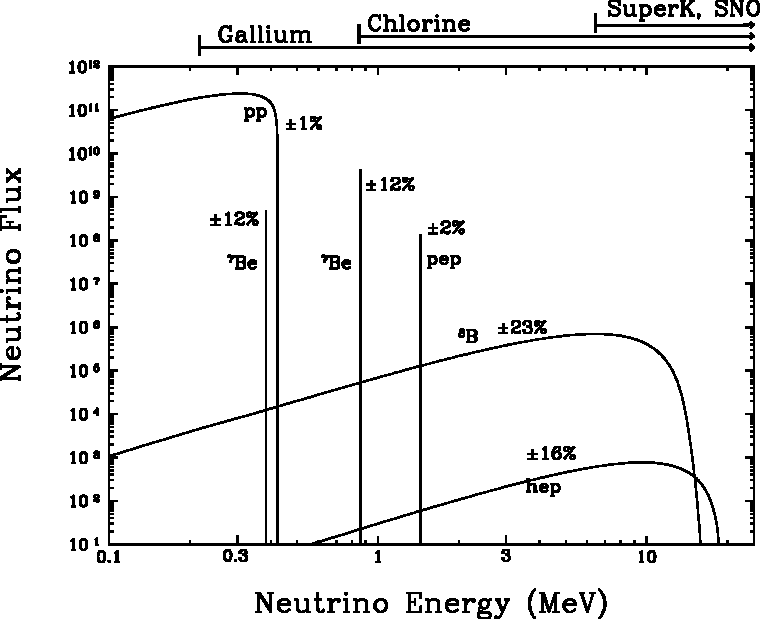
\includegraphics[width=0.6\textwidth]{pics/BahcallNuFlux.pdf}
	\caption{The predicted neutrino flux from the solar standard model~\cite{Bahcall:2004mz}.
		The threshold energies of major solar neutrino experiments are shown for comparison.}
	\label{fig:solar_nu_flux}
\end{figure}

The second astrophysical source of neutrinos ever identified was the Supernova (SN) explosion SN1987A %
which occured on the 23\tapi{rd} of February, 1987, in the Large Magellanic Cloud.
It was the only SN explosion which was detected through its neutrino emission.
Supernova explosions are another important source of neutrinos.
Historically, SN are classified by their spectral characteristics near maximal luminosity.
This is dictated by the composition of the progenitor star.
The main subdivision is between spectra with or without hydrogen lines, respectively called %
type II and type I.
Further classification of type I SN comes from the presence of silicon and helium.
Type Ia SN, the spectrum of which shows Si strong lines, is the only SN type that is not accompanied %
by a substantial neutrino emission.
This is because the mechanism of explosion comes from the accretion white dwarf to the point where %
the pressure of the degenerate electron gas can no longer sustain the gravitational pull.
The limit is known as \emph{Chandrasekhar limit} and it is around 1.4\,$M_\odot$.
When the white dwarf collapses, the fusion of carbon and oxygen heavy nuclei is activated %
and an enormous quantity of energy is freed in thermonuclear processes.

\begin{figure}
	\centering
	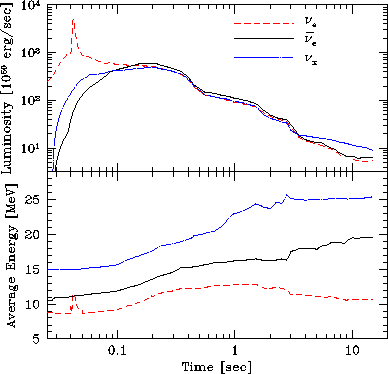
\includegraphics[width=0.5\textwidth]{pics/SN_burst.pdf}
	\caption{Time and energy profile of the predicted neutrino flux from a Supernova core-collapse of %
		mass $M \simeq 20\,M_\odot$~\cite{Totani:1997vj}.
		Other neutrino flavours than $\nu_e$ and $\cj{\nu}_e$ are collectively represented by %
		$\nu_X = (\nu_\mu + \cj{\nu}_\mu + \nu_\tau + \cj{\nu}_\tau) / 4$.}
	\label{fig:sn_nu_flux}
\end{figure}

On the other hand, the supernovae of type Ib, Ic, and II explode via core-collapse, %
libearting an intense flux of neutrinos..
Old stars with a mass $M \gtrsim 8\,M_\odot$ and $M \lesssim 40\,M_\odot$ tend to stratify %
in layers of elements undergoing fusion, with the lightest (H) in the outer shell burning into heavier nuclei %
(He, C, Ne, Mg, Si, ...) up to iron at the core.
After carbon ignition, the neutrino luminosity of the star comes mainly from a long silicon burning phase.
The \emph{pre-supernova} neutrinos make up roughly 1\,\% of the total energy that is emitted during the star's core-collapse.
At this stage, the gravitational pressure is balanced overall by the thermonuclear energy released in each shell, %
but in the Fe core for which esothermic reactions are not allowed.
The mass of the core is sustained by the pressure of degenerate relativistic electrons, %
which is reduced by photodissociation of iron 
\begin{equation}
	\gamma +  {}^{56}\text{Fe} \to 13\,\alpha + 4\,n - 124.4\,\text{MeV}\ ,
\end{equation}
and electron capture with neutrinos escaping the supernova
\begin{equation}
	e^- + p \to n + \nu_e\ .
\end{equation}
Once the Fermi pressure is no longer sufficient to contrast the core, this collapses %
and the increase in temperature accelerates photodissociation and electron capture in a positive feedback reaction.
The density of the core, however, increases until when neutrinos from electron capture are trapped inside %
and so collapse becomes an adiabatic process.
The free-falling core is finally stopped by the pressure of degenerate non-relativistic nucleons.
The abrut halt causes a shock wave that propagates to the outer parts of the core and slows down the imploding mantle.
As the shock propagates through the infalling dense matter of the outer core,
The energy of the shock is dissipated by the photodissociation of nuclei into nucleons, %
leading to an intensification of the electron capture rate thanks to the copious number of free protons.
The electron neutrinos pile up behind the opaque wave until the shock reaches a layers of lower density 
and the $\nu_e$ are released in a few millisecond in what is called \emph{neutronisation burst}, %
carrying away around \np{e50}\,erg.
In most scenarios, the shock wave stalls and the bounce mechanism from the core alone is not enough to cause an explosion.
The remnant of the core, which is forming a proto-neutron star, can revive the shock if its mass is large enough.
In the hot core, numerous neutrinos are produced in all flavours by electron-positron annihilation, %
electron-nucleon and nucleon-nucleon bremsstrahlung, and electron neutrinos from electron or positron capture.
These neutrinos get trapped between the core and the mantle regions with a density high enough such that %
their mean free path is smaller than the supernova radius.
This region, known as \emph{neutrinosphere}, depends on the $\nu$ energies and flavours %
and emits a thermal flux of neutrinos the energy of which could revive the shock up to explosion.
The luminosity of neutrinos in this phase does not peak as for the neutronisation burst, %
but presents a long hump on a time scale of a few seconds, as seen in \reffig{fig:sn_nu_flux}.
The average energies are typically higher for muon and tau neutrino, since they are produced in deeper %
region of the SN, the values of which strongly depend on the model (see for example \refrefs{Totani:1997vj, Nakazato:2012qf, Tamborra:2014hga}).
These and the energies for electron neutrinos and antineutrinos usually range between 10\,MeV and 30\,MeV.


\subsection{Atmospheric and accelerator neutrinos}
\label{sec:nu_atm_acc}

Atmospheric neutrinos are generated by the interactions of cosmic rays with the Earth's atmosphere.
Primary cosmic rays are mainly composed by energetic protons or heavier nuclei, originated from the Sun %
or outside the solar system.
Their interactions with nuclei in the atmosphere produces pseudo-scalar mesons such as pions and kaons, %
which rapidly decay into charged leptons and neutrinos.
Due to helicity suppression, the two-body decays of $\pi^\pm$ and $K^\pm$ favour the muon channel
\begin{align}
	\pi^\pm &\rightarrow \mu^\pm + \overset{(-)}{\nu_\mu} \\
	K^\pm &\rightarrow \mu^\pm + \overset{(-)}{\nu_\mu} \ .
\end{align}
The muon itself decays with a relatively longer lifetime releasing two neutrinos per decay:
\begin{align}
	\mu^+ &\rightarrow e^+ + \nu_e + \cj{\nu}_\mu \\
	\mu^- &\rightarrow e^- + \cj{\nu}_e + \nu_\mu \ .
\end{align}
At sufficient low energies of $E \lesssim 1$\,GeV, all of the muons decay before reaching the ground and %
so the neutrino fluxes follow the proportions of neutrino flavours 
\begin{align}
	\phi_{\nu_e} : \phi_{\nu_\mu} &= 1 : 2 \\
	\phi_{\nu_\mu} : \phi_{\cj{\nu}_\mu} &= 1 : 1 \\
	\phi_{\nu_e} : \phi_{\cj{\nu}_e} &= \phi_{\mu^+} : \phi_{\mu^-} \ .
\end{align}
At higher energies, the amount of mouns hitting the ground before decaying increases, changing the ratio between flavours.
The energy range of primary cosmic rays goes from 200\,MeV up to about \np{e20}\,eV, as it is shown in \reffig{fig:CR_flux}.
The isotropy in the angular distribution of cosmic rays and their energies suggest that they are produced mostly %
outside the solar system.
Above a few GeV, the cosmic ray spectrum approximately follows $E^{-2.7}$ apart in the region between %
\np{e15.5}\,eV and \np{e17.7}\,eV where the behaviour is $E^{-3.0 \sim -3.3}$.
The maximum theoretical limit is near \np{e20}\,eV~\cite{Abraham:2008ru}, after which the spectrum is suppressed because of %
the interactions of the cosmic rays with the cosmic microwave background, also known as %
Greisen-Zatsepin-Kuzmin (GZK) cutoff~\cite{Greisen:1966jv, Zatsepin:1966jv}.

\begin{figure}
	\begin{minipage}[t]{0.4\textwidth}
		\centering
		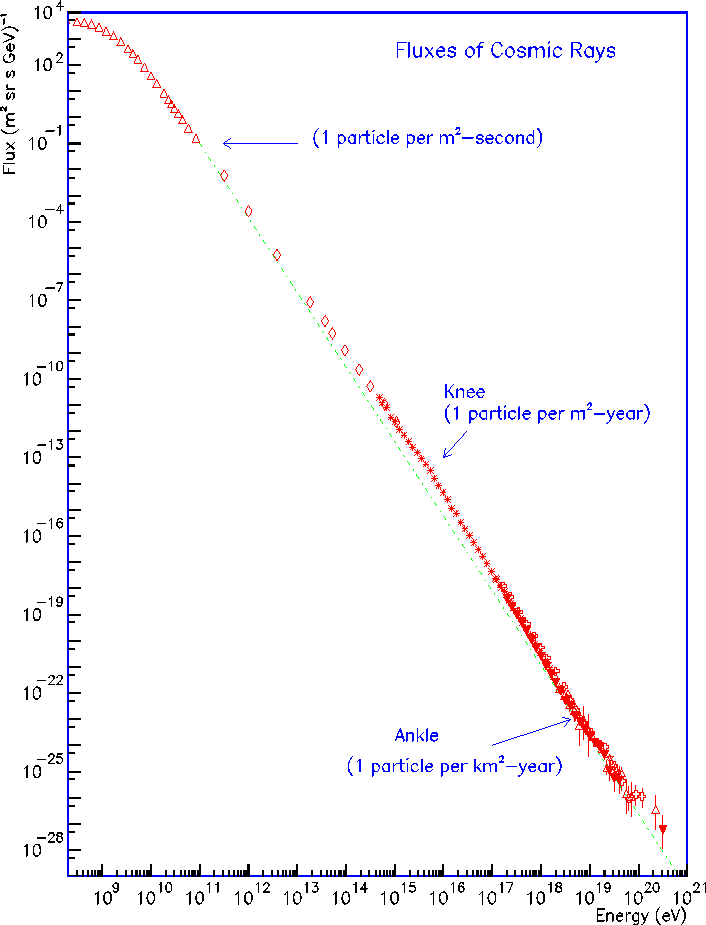
\includegraphics[width=0.9\textwidth]{pics/CR_flux.pdf}
		\captionof{figure}{Measurement of cosmic rays over the entire energy spectrym, %
			where the change of energy dependance is visible (\emph{knee})~\cite{Anchordoqui:2002hs}.}
		\label{fig:CR_flux}
	\end{minipage}
	\hfill
	\begin{minipage}[t]{0.6\textwidth}
		\centering
		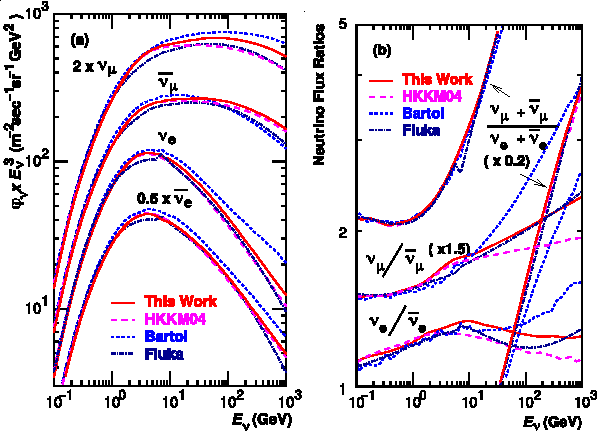
\includegraphics[width=\textwidth]{pics/honda_flux.pdf}
		\captionof{figure}{Prediction of atmospheric neutrinos from~\cite{Honda:2004yz}.}
		\label{fig:honda_flux}
	\end{minipage}
\end{figure}

The neutrinos are therefore produced isotropically around the atmosphere with energies up to a few hundreds of TeV, %
peaking at tens of GeV, even though the energy distribution is flavour dependent.
Despite the production point of neutrinos varies in altitude, with a most probables value around 15\,km,
for an experiment on the Earth's surface, neutrinos are coming from all directions with the flight path depending %
on the zenith angle to the origin.
This means that the distance travelled by atmospheric neutrinos varies from a minimum of a few kilometers %
to a maximum equal to the Earth's diameter, \np{1.2e4}\,km.
It was observed by the Super-Kamiokande experiment that the ratio of flavours of neutrinos from %
positive and negative zenith angle were different, implying the presence of neutrino oscillation~\cite{Fukuda:1998mi}.
A correct prediction of the atmospheric flux becomes instrumental in studying oscillation physics; %
computational-intensive 3D simulations have reached state-of-the-art precision with negligible statistical errors %
also thanks to the implementation of gemagnetic models~\cite{Honda:2004yz, Honda:2006qj}.

Atmospheric neutrinos provide an invaluable source for studying the properties of neutrinos, %
such as the squared mass differences and the mixing angles.
However, the uncertainty on the path lengths of neutrinos from production to detection can downgrade %
the precision of the measurement.
Man-made accelerator facitilies try to overcome this limitation.
Neutrino beams are derived from a similar mechanism that generates atmospheric neutrinos.
A proton beam hitting a fixed target typically yields a large number of pions and kaons, %
and also heavier mesons, the amount of which depends on the energy of the protons and the choice of the target.
All these secondary particles decay leptonically or semi-leptonically via CC weak interactions thus creating a neutrino beam.
Pions and kaons principally decay into $\nu_\mu$ because two-body electronic modes are disfavoured %
by helicity suppression.
Muons decay in turn into equal numbers of $\nu_e$ and $\cj{\nu}_\mu$.
Other production sources of $\nu_e$ are the three-body decays of $K^0$ and $K^+$.
The parentage composition of the Booster Neutrino Beam flux~\cite{AguilarArevalo:2008yp} %
is shown in \reffig{fig:bnb_flux},
Above the neutral kaon mass, the first sizeable source of neutrino is given by the $D_s$ meson, %
for which helicity suppression again favours the production of heavy charged-leptons, %
and so $\tau$~leptons and $\nu_\tau$ are more likely to be emitted than the other flavours.
Each of the subsequent $\tau^+$ decays produces a $\cj{\nu}_\tau$.
The production of $D_s$ meson, however, requires very energetic proton beams and therefore %
for practical reaons this constribution is disregarded.

\begin{figure}
	\begin{minipage}[t]{0.48\textwidth}
		\centering
		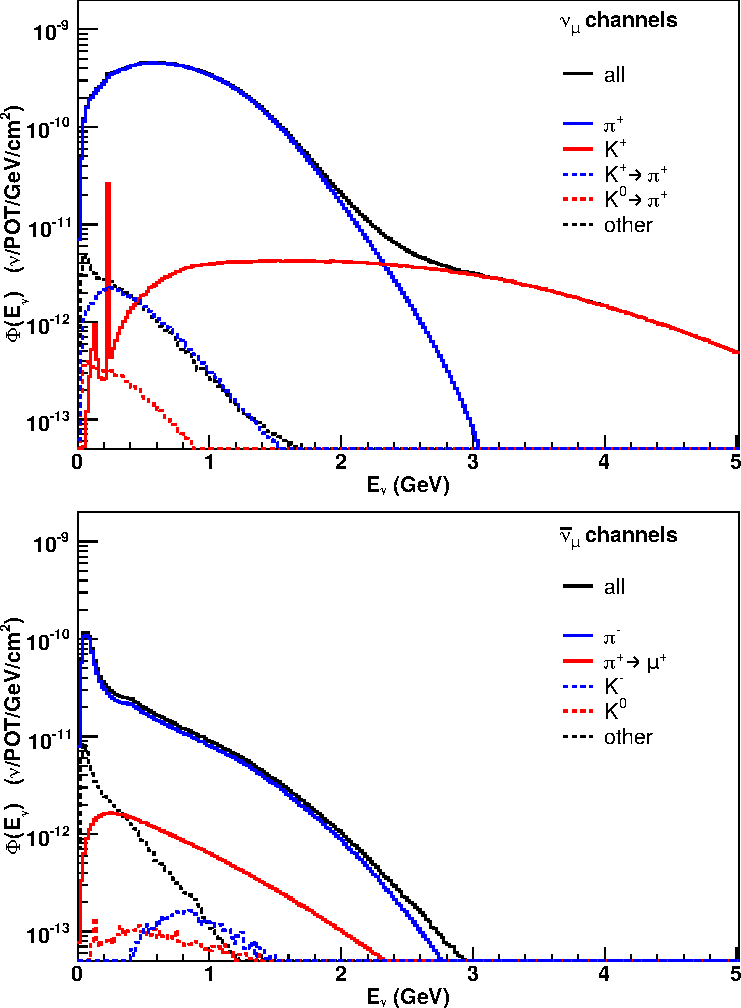
\includegraphics[width=\textwidth]{pics/bnb_flux.pdf}
		\captionof{figure}{Prediction of the $\nu_\mu$ and $\cj{\nu}_\mu$ fluxes at the %
			Booster Neutrino Beam~\cite{AguilarArevalo:2008yp}.
			The contributions from the parent particles are highlighted.}
		\label{fig:bnb_flux}
	\end{minipage}
	\hfill
	\begin{minipage}[t]{0.48\textwidth}
		\centering
		\raisebox{3.0em}{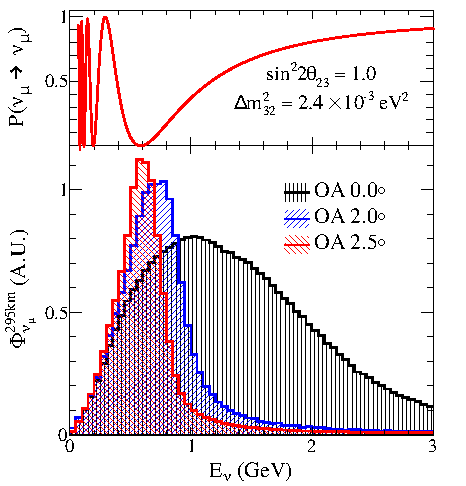
\includegraphics[width=\textwidth]{pics/t2k_flux.pdf}}
		\captionof{figure}{Prediction of the $\nu_\mu$ flux at T2K~\cite{Abe:2012av}, %
		       showing the profile at different off-axis angles (OA).
		       At $2.5^\circ$ from the axis, the energy distributions peaks %
		       in correspondence of a minimum for the $\nu_\mu$ disappearance probability.}
		\label{fig:t2k_flux}
	\end{minipage}
\end{figure}



The energy and angular distributions of the neutrino beam reflect the kinematic properties of %
the parent particles, which are in turn produced with a variety of angles and energies.
The wide angular distribution might not be suitable for neutrino experiments, which require very high statistics.
To improve the quality of the nuetrino beam, a focusing system is typically put into place %
by partially surrounding the target with one or more pulsed toroidal electromagnets, called \emph{horns}.
The horns are activated with currents of hundreds of kilo-Ampere for a few microseconds %
in coincidence with the protom beam arriving at the target.
Within the horn cavity, the pulse creates a magnetic field that decreases %
radially with respect to the axis of the horn, meaning that the peak intensitity of the magnetic field %
is reached at the inner regions of the toroid.
Despite the optimal design of the horn, kaons and short-lived mesons cannot be deflected as efficiently %
as pions and muons.
This results in a intrinsic spread of the neutrino beam.
In certain cases, the neutrino experiment is located off the axis of the beam, as in T2K~\cite{Abe:2012av} %
and NO$\nu$A~\cite{Ayres:2004js}.
At angles $\theta > 0$ the energy of the neutrino becomes independent of the %
energy of the parent meson neutrinos and the energy distribution is roughly monochromatic~\cite{Beavis_Carroll_Chiang_1995}.
This charactheristic is favourable in oscillation experiment, in which the ratio between baseline and %
neutrino energy is fixed and known, as shown in \reffig{fig:t2k_beam}.


\section{Neutrino interactions}
\label{sec:neutrino_interactions}

Neutrino interactions in their flavour states are described by \refeqs{eq:lepton_cc}{eq:lepton_nc}.
Replacing the values of $g^\nu_V$ and $g^\nu_A$ for a neutrino, the relevant lagrangian terms are
\begin{align}
	%\label{eq:real_lepton_cc}
	\mathcal{L}_{\text{CC},\nu} &= -\frac{g}{2\sqrt{2}}\ 	      %
	\sum_{\alpha=e,\mu,\tau} \cj{\nu}_\alpha \sh{W} (1-\gamma^5) \ell_\alpha + \text{h.c.} \\
	%\label{eq:real_lepton_nc}
	\mathcal{L}_{\text{NC},\nu} &= -\frac{g}{4\cos\vartheta_\text{W}}\ %
	\sum_{\alpha=e,\mu,\tau} \cj{\nu}_\alpha \sh{Z} (1-\gamma^5) \nu_\alpha \ .
\end{align}
For energies below the $W$ and $Z$ mass, the allowed tree-level interactions involving at least one neutrino %
are any allowed variation of the processes represented in \reffig{fig:neutrino_tree}.
The vector bosons cannot be produced on-shell and so their field operator must contract with some other external field.
The amplitudes of the processes shown in \reffig{fig:neutrino_tree} are
\begin{align}
	i \mathcal{M}_\text{CC} &= i\, \frac{g^2}{8}\ \cj{u}_{\ell_\alpha} \gamma^\mu (1-\gamma^5)\, u_{\nu_\alpha}
						    \,\frac{\eta_{\mu\nu}}{k^2 - m_W^2+i\varepsilon}
						    \,\cj{u}_{f_2} \gamma^\nu (1-\gamma^5)\,V_{12}\, u_{f_1} \\
	i \mathcal{M}_\text{NC} &= i\, \frac{g^2}{8\cos\vartheta}\ \cj{u}_{\nu_\alpha} \gamma^\mu (1-\gamma^5)\, u_{\nu_\alpha}
						    \,\frac{\eta_{\mu\nu}}{k^2 - m_Z^2+i\varepsilon}
						    \,\cj{u}_{f} \gamma^\nu (g^f_V-g^f_A\gamma^5) u_{f}\ ,
\end{align}
where $k$ is the momentum of the propagator and $V_{12}$ a possible mixing between generic fermions $f_1$ and $f_2$.
Because of the typical energies involved, the momentum propagating between the particles is small %
compared to the masses of the intermediate bosons and therefore their mass can be factorised out, %
resulting in the four-point interactions
\begin{align}
	\label{eq:fermi_cc}
	i \mathcal{M}_\text{CC} &\simeq i\,  \frac{G_F^2}{\sqrt{2}}\ \cj{u}_{\ell_\alpha} \gamma^\mu (1-\gamma^5)\, u_{\nu_\alpha}
						    \,\cj{u}_{f_2} \gamma^\mu (1-\gamma^5)\,V_{12}\, u_{f_1} \\
	\label{eq:fermi_nc}
	i \mathcal{M}_\text{NC} &\simeq i\,  \frac{G_F^2}{\sqrt{2}}\ \cj{u}_{\nu_\alpha} \gamma^\mu (1-\gamma^5)\, u_{\nu_\alpha}
						    \,\cj{u}_{f} \gamma^\mu (g^f_V-g^f_A\gamma^5) u_{f}\ ,
\end{align}
where the relation in \refeq{eq:magic_ratio} was used and a new constant was introduced 
\begin{equation}
	\label{eq:fermi_const}
	\frac{G_F}{\sqrt{2}} = \frac{g^2}{8\,m_W^2}\ .
\end{equation}
The constant in \refeq{eq:fermi_const} is called Fermi's constant and the interactions %
can be described by effective four-point Lagrangians.
%\begin{align}
%	\mathcal{L}_\text{eff, CC} &= - \frac{G_F}{\sqrt{2}} \qty[\cj{\ell}_\alpha \gamma^\mu(1-\gamma^5)\nu_\alpha] %
%							     \qty[\cj{f}_2\gamma_\mu(1 - \gamma^5) f_1] \\
%	\mathcal{L}_\text{eff, CC} &= - \frac{G_F}{\sqrt{2}} \qty[\cj{\nu}_\alpha \gamma^\mu(1-\gamma^5)\nu_\alpha] %
%							     \qty[\cj{f}\gamma_\mu(g^F_V - g^F_A \gamma^5) f]
%\end{align}
						    
\begin{figure}
	\centering
	\medskip
	\begin{fmffile}{neutrino_CC}
		\begin{fmfgraph*}(80,60)
			\fmfleft{f1,nu}
			\fmfright{f2,ell}
			\fmf{fermion}{nu,v1,ell}
			\fmf{fermion}{f1,v2,f2}
			\fmf{photon, label=$W$}{v1,v2}
			\fmflabel{$f_1$}{f1}
			\fmflabel{$f_2$}{f2}
			\fmflabel{$\nu_\alpha$}{nu}
			\fmflabel{$\ell_\alpha$}{ell}
		\end{fmfgraph*}
	\end{fmffile}
	\qquad
	\raisebox{2.5em}{,}
	\qquad
	\begin{fmffile}{neutrino_NC}
		\begin{fmfgraph*}(80,60)
			\fmfleft{f1,nu1}
			\fmfright{f2,nu2}
			\fmf{fermion}{nu1,v1,nu2}
			\fmf{fermion}{f1,v2,f2}
			\fmf{photon, label=$Z$}{v1,v2}
			\fmflabel{$f$}{f1}
			\fmflabel{$f$}{f2}
			\fmflabel{$\nu_\alpha$}{nu1}
			\fmflabel{$\nu_\alpha$}{nu2}
		\end{fmfgraph*}
	\end{fmffile}
	\bigskip
	\caption{Generic CC (right) and NC (left) tree-level interactions with neutrinos involved.
		Note that these diagrams have illustration purpose only, and that's why time flow convention is not respected. }
	\label{fig:neutrino_tree}
\end{figure}

In the following sections we will review the most important neutrino interactions with matter, %
from low to higher energies.

\subsection{Coherent elastic neutrino--nucleus scattering}
\label{sec:cevns}

The coupling of neutrinos to the $Z$ boson opens the possibility of a coherent interactions %
with all the nucleons in an atomic nucleus~\cite{Freedman:1973yd}.
This possibility would exist only as long as the momentum exchanged remained significantly smaller than the inverse of the nuclear
size (Fig. 1A), effectively restricting the process to neutrino energies below a few tens of MeV.
The enhancement to the probability of interaction (scattering cross-section) would however be
very large when compared to interactions with isolated nucleons, approximately scaling with the
square of the number of neutrons in the nucleus (2, 3). For heavy nuclei and sufficiently intense
neutrino sources, this can lead to a dramatic reduction in detector mass, down to a few
kilograms.

\subsection{Neutrino--electron scattering}
\label{sec:elastic_scattering}

The easiest interaction to study between neutrinos and matter components at low energies %
is the neutrino--electron elastic scattering
\begin{equation}
	\overset{(-)}{\nu}_\alpha + e^- \rightarrow \overset{(-)}{\nu}_\alpha + e^-\ .
\end{equation}
For the electron neutrino $\nu_e$, both CC and NC interactions are allowed and %
for the electron antineutrino $\cj{\nu}_e$ the $s$-channel and $t$-channel diagrams are swapped,
whereas for $\alpha = \mu, \tau$ only neutral-current interactions exist.
%The respective Feynman diagrams are shown in Fig.~\ref{fig:nescat} and~\ref{nutscat}.
%The effective lagrangian 
%\begin{align}
%	\mathcal{L}_\mathrm{eff}(\nu_e e^- \rightarrow \nu_e e^-) &= - \frac{G_F}{\sqrt{2}} %
%	[\overline{\nu_e}\gamma^\mu(1-\gamma^5)\nu_e][\bar{e}\gamma_\mu((1+g_V^l)-(1+g_A^l)\gamma^5)e] \\
%	\mathcal{L}_\mathrm{eff}(\nu_\alpha e^- \rightarrow \nu_\alpha e^-) &= - \frac{G_F}{\sqrt{2}} %
%	[\overline{\nu_\alpha}\gamma^\mu(1-\gamma^5)\nu_\alpha][\bar{e}\gamma_\mu(g_V^l-g_A^l)\gamma^5)e] %
%	\quad (\alpha = \mu,\tau)\,.
%\end{align}
Using the effective four-point Lagrangians, one can calculate the differential cross-sections in the laboratory frame %
with an initial electron at rest:
\begin{equation}
	\label{eq:nu_elastic_xsec}
	\dv{\sigma}{q^2} = \frac{G_F^2}{\pi} \qty[\kappa_1^2 + \kappa_2^2 
		\qty(1 - \frac{q^2}{2\,(p_\nu \cdot p_e)} )^2 - \kappa_1\, \kappa_2\, m_e^2\, \frac{q^2}{2\, (p_\nu \cdot p_e)^2} ] \ ,
\end{equation}
where $-q^2 = t$ and the quantities $\kappa_1$ and $\kappa_2$ %
depend on the neutrino flavour and embeds CC and NC contributions.
Using the vector and axial coupling of \refeq{eq:gv_ga} they read
\begin{align*}
	&\kappa_1^{\nu_e} = \kappa_2^{\cj{\nu}_e} = 1 + \frac{g_V^\ell + g_A^\ell}{2} = \frac{1}{2} + \sin^2\vartheta_W \\
	&\kappa_2^{\nu_e} = \kappa_1^{\cj{\nu}_e} = \frac{g_V^\ell - g_A^\ell}{2} = \sin^2\vartheta_W \\
	&\kappa_1^{\nu_{\mu,\tau}} = \kappa_2^{\cj{\nu}_{\mu,\tau}} = \frac{g_V^\ell + g_A^\ell}{2} = -\frac{1}{2} + \sin^2\vartheta_W \\
	&\kappa_2^{\nu_{\mu,\tau}} = \kappa_1^{\cj{\nu}_{\mu,\tau}} = \frac{g_V^\ell - g_A^\ell}{2} = \sin^2\vartheta_W \ .
\end{align*}

The variable $t$ is the squared difference between the four-momentum of the initial and final electrons, 
and denoting $T_e = E_e - m_e$ as the kinetic energy of the outgoing electron, we see that
\begin{equation}
	-t = q^2 = 2\,m_e\,T_e\ .
\end{equation}
With some simple kinematics the kinetic energy is found to be
\begin{equation}
	T_e = \frac{2\,m_e\,E_\nu^2 \cos^2 \theta}{(m_e + E_\nu)^2 - E_\nu^2 \cos^2\theta}\ ,
\end{equation}
and so the differential cross-section in \refeq{eq:nu_elastic_xsec} can be given as a function of the %
electron scattering angle $\theta$ with respect to the incoming neutrino with energy $E_\nu$:
\begin{align}
	\dv{\sigma}{\cos\theta} =&\ \frac{2 G_F^2 m_e}{\pi} %
			\frac{4 E_\nu^2 (m_e+E_\nu)^2 \cos \theta}{\qty[(m_e+E_\nu)^2-E_\nu^2 \cos^2 \theta ]^2} \quad \times \notag \\
			&\qty[g_1^2 + g_2^2\qty(1 - \frac{2 m_e E_\nu \cos^2 \theta}{(m_e+E_\nu)^2-E_\nu^2 \cos^2 \theta} )^2
		- g_1\, g_2\, \frac{2m_e^2 \cos^2 \theta}{(m_e+E_\nu)^2-E_\nu^2 \cos^2 \theta}]\ .
\end{align}

\subsection{Neutrino scattering with nucleons}

Neutrinos can also interact with hadrons in matter, namely proton and neutrons, %
as the quark components of these baryons couple to the $W$ and $Z$ vector bosons according to %
the currents of \refeqs{eq:real_quark_cc}{eq:real_quark_nc}.
The compoEven though
In general, these processes can be categorised according to the momentum transfer.
At small $q^2$, elastic interactions dominate and may be brought about by both charged and neutral currents.
When this occurs via neutral currents, all flavour of neutrinos and anti-neutrinos can scatter off %
both neutrons and protons in what is referred to as ``NC elastic'' scattering.
The process is:
\begin{align}
	\nu_\alpha + N \rightarrow \nu_\alpha + N \\
	\bar\nu_l + N \rightarrow \bar\nu_l + N\ ,
\end{align}

Once neutrinos acquire sufficient energy they can also undergo the analogous charged current interactions, %
called ``quasi-elastic'', due to the fact that the recoiling nucleon changes its charge and mass transfer occurs.
The processes are
\begin{align}
	\nu_l + n &\rightarrow p + l^- \\
	\bar\nu_l + p &\rightarrow n + l^+ \ ,
\end{align}
with $l=e, \mu, \tau$.
For the muonic neutrino with energy below one GeV, the CCQE is the dominant interaction, event though the %
cross-section plateaus at higher energies, as the available $Q^2$ increases: it becomes increasingly unlikely %
for the nucleon to remain intact.

The physics behind the CC quasi-elastic processes is more complicated.
The differential cross-section for the scattering in the laboratory frame is given by
\begin{equation}
	\label{eq:cc_xsec_q}
	\frac{\mathrm{d} \sigma_{CC}}{\mathrm{d}Q^2} = \frac{G_F^2 |V_{ud}|^2 m_N^4}{8\pi (p_\nu \cdot p_N)^2} %
	\bigg [A(Q^2) \pm B(Q^2) \frac{s-u}{m_N^2} + C(Q^2) \frac{(s-u)^2}{m_N^4} \bigg]\,,
\end{equation}
where the plus sign refers to the $N = n$ interactions, while the minus sign to $N = p$.

\begin{equation}
	\label{eq:cc_xsec_t}
	\frac{\mathrm{d} \sigma_{CC}}{\mathrm{d}\cos\theta} = -\frac{G_F^2 |V_{ud}|^2 m_N^2}{4\pi} \frac{p_l}{E_\nu} %
	\bigg [A(Q^2) \pm B(Q^2) \frac{s-u}{m_N^2} + C(Q^2) \frac{(s-u)^2}{m_N^4} \bigg]\,,
\end{equation}

The functions $A(Q^2)$, $B(Q^2)$, and $C(Q^2)$ depends on the nucleon form-factors in the following way:
\begin{align}
	\begin{split}
		\label{eq:A(Q)}
		A &= \frac{m_l^2+Q^2}{m_N^2} \bigg\{ \bigg(1+\frac{Q^2}{4m_N^2}\bigg) G_A^2 - \bigg(1-\frac{Q^2}{4m_N^2}\bigg) %
		\bigg(F_1^2 - \frac{Q^2}{4m_N^2}F_2^2 \bigg) +\frac{Q^2}{m_N^2} F_1 F_2 \\
		&\qquad- \frac{m_l^2}{4m_N^2} %
		\bigg[ (F_1+F_2)^2+(G_A+2G_P)^2-\frac{1}{4}\bigg(1+\frac{Q^2}{4m_N^2}\bigg) G_P^2 \bigg] \bigg\}\, 
	\end{split}\\
	\label{eq:B(Q)}
	B &= \frac{Q^2}{m_N^2} G_A (F_1+F_2)\,\\
	\label{eq:C(Q)}
	C &= \frac{1}{4} \big (G_A^2 +F_1^2+\frac{Q^2}{4m_N^2}F_2^2\big)\,.
\end{align}

The form factors $F_1(Q^2)$, $F_2(Q^2)$, $G_A(Q^2)$, and $G_P(Q^2)$ are called, respectively, \emph{Dirac}, %
\emph{Pauli}, \emph{axial}, and \emph{pseudoscalar} weak charged-current form factors of the nucleon.
These functions of $Q^2$ describe the spatial distributions of electric charge and current inside the nucleon %
and thus are intimately related to its internal structure.

CCQE interactions are particularly important to neutrino physics for mainly two reasons:
\begin{itemize}
	\item measurements of the differential cross-section in Eq.~\ref{eq:cc_xsec_q} give information on the %
		nucleon form-factors, which are difficult to measure; 
	\item their nature as two-body interactions enable the kinematics to be completely reconstructed, %
		and hence the initial neutrino energy determined which is critical for measuring the oscillation parameters.
\end{itemize}

In fact, if the target nucleon is at rest, at least compared to the neutrino energy, %
then this can be calculated as:
\begin{equation}
	E_\nu = \frac{m_n E_l + \frac{1}{2}\big ( m_p^2-m_n^2-m_l^2)}{m_n - E_l+p_l \cos \theta_l}\,,
\end{equation}
where the measurement of the momentum, $p_l$ and the angle with respect to the neutrino, $\theta_l$, of the %
outgoing charged lepton are only required.

Similar calculations can be made for the NCQE scatterings.
The cross-sections have the same form as the CC cross-sections in Eq.~\ref{eq:cc_xsec_q} and ~\ref{eq:cc_xsec_t}, %
without the mixing term $|V_{ud}|^2$ and with the proper nucleon form factors.
Since the values of the electromagnetic form factors, $F_1$ and $F_2$, are reasonably well known and the part %
in Eq.~\ref{eq:A(Q)} containing $G_P$ can be often neglected, thanks to the different mass magnitudes of %
leptons and nucleons, the axial form factor, $G_A$, can be determined through measurements of the charged-current %
quasielastic scattering processes.
On the contrary, measurements of the neutral-current elastic scattering cross-section give information %
on the \emph{strange} form factors of the nucleon, whose main contribute comes from the strange quark.

The low $Q^2$ region also presents an inelastic scattering contribution mostly affected by resonance production, %
where the nucleon is excited into a baryonic resonance before decaying.
At high $Q^2$, inelastic scattering is dominated by deep inelastic scattering (DIS), because the neutrino can scatter %
directly off a constituent quark, fragmenting the original nucleon.
In between these extreme scenarios, an additional contribution comes from interactions where the hadronic %
system is neither completely fragmented nor forms a recognisable resonance.
These interactions are referred to as ``shallow inelastic scattering'', and there is no clear model for dealing %
with them.

